%%%%%%%%%%%%%%%%%%%%%%%%%%%%%%%%%%%%%%%%%
% Journal Article
% LaTeX Template
% Version 2.0 (February 7, 2023)
%
% This template originates from:
% https://www.LaTeXTemplates.com
%
% Author:
% Vel (vel@latextemplates.com)
%
% License:
% CC BY-NC-SA 4.0 (https://creativecommons.org/licenses/by-nc-sa/4.0/)
%
% NOTE: The bibliography needs to be compiled using the biber engine.
%%%%%%%%%%%%%%%%%%%%%%%%%%%%%%%%%%%%%%%%%
% Modified by:
% Pakorn Wangsuekul (joe@ai.iit.tsukuba.ac.jp)
%
% Version 2.1 (July 9, 2023)
% Version 2.2 by Hiroaki Yano (July 11, 2023) 
% Version 2.3 (July 13, 2023)
%%%%%%%%%%%%%%%%%%%%%%%%%%%%%%%%%%%%%%%%%

%----------------------------------------------------------------------------------------
%	PACKAGES AND OTHER DOCUMENT CONFIGURATIONS
%----------------------------------------------------------------------------------------

\documentclass[
	a4paper, % Paper size, use either a4paper or letterpaper
	10pt, % Default font size, can also use 11pt or 12pt, although this is not recommended
	% unnumberedsections, % Uncomment to remove section numbering
	% twoside, % Uncomment to enable two side traditional mode where headers and footers change between odd and even pages
]{LTJournalArticle}

\addbibresource{bibliography.bib} % BibLaTeX bibliography file

\headerleft{Hochschule Kaiserslautern University of Applied Sciences} % Left running head
\headerright{2023-24 Mechanical Engineering/Mechatronics} % Right running head: Student ID and Name

\footertext{} % Text to appear in the footer, leave this command empty for no footer text

\setcounter{page}{1} % Page number of the first page, set this to a higher number if the article is to be part of a larger publication

%----------------------------------------------------------------------------------------
%	TITLE SECTION
%----------------------------------------------------------------------------------------

% Report title
\title{Comparative Study on Battery and Hydrogen PEM Fuel Cell Powered Hybrid Propulsion System under Different Driving Conditions} % Article title, max 3 lines recommended

% Author's name
\author{
	A Kalyan Prudhvi, Amit Kumar Pai, Zubair Hussain Hamid\ \fontsize{9pt}{12pt}\selectfont Master's Program in Mechanical Engineering/Mechatronics
}

% Supervisor name and Laboratory name
\date{
        Supervised by: Prof. Dr.-Ing. Peter Heidrich %\hfill Insert Laboratory Name Here
}

% Abstract (approx. 100 words) and keywords (approx 5 words)
\renewcommand{\maketitlehookd}{%
	\begin{abstract}
            \textbf{Abstract:} 
The persistent rise in atmospheric CO\textsubscript2 levels has spurred urgent calls for mitigating climate change impacts. In response, the European Commission has outlined ambitious targets for 2030 to curtail greenhouse gas emissions and promote renewable energy adoption. Addressing these challenges, fuel cell vehicles (FCVs) have emerged as a promising alternative to conventional internal combustion engine vehicles. Fuel Cell Automotive Trainer (FCAT) is a comprehensive hybrid propulsion system that integrates both battery and hydrogen proton exchange membrane (PEM) fuel cell technologies to simulate FCVs.
Through this paper we delve into the behaviour and capabilities of fuel cell along with hybrid propulsion system through a series of experimental simulations. The study encompasses of two main experiments. Firstly, the examination of a stack of fuel cells to assess system performance under various controlled conditions is carried out. Secondly, the evaluation of a hybrid propulsion system with the FCAT apparatus under various driving conditions is conducted. Through data acquisition and analysis, the paper elucidates the synergistic operation of battery and PEMFC components within the hybrid propulsion system.

Graphical representations of simulated driving scenarios illustrate the dynamic interplay between energy sources and load demands, elucidating the nuanced operational dynamics of hybrid energy systems in achieving optimal performance. This research paper, emphasizes the role of FCAT in investigating hybrid energy systems and its implications for sustainable transportation.

The results show that using the fuel cell as the only energy source will not fulfil the requirements of various operating conditions. In a hybrid propulsion system, the two energy sources complement each other with the hydrogen fuel cell supplying sufficient energy for a constant speed drive and with the battery fulfilling the peak energy demand when rapidly accelerating. This is further supplemented by the recharging of the battery from the hydrogen fuel cell in idle state. The results also demonstrate that the hydrogen PEM fuel cells perform well at optimal temperatures [8].  

.
            
            \textbf{Keywords:} Hydrogen Fuel Cell, Hybrid Propulsion System, Proton Exchange Membrane, Fuel Cell Automotive Trainer
	\end{abstract}
}

%----------------------------------------------------------------------------------------

\begin{document}

\maketitle % Output the title section

%----------------------------------------------------------------------------------------
%	ARTICLE CONTENTS
%----------------------------------------------------------------------------------------

\section{Introduction}

The ongoing escalation in atmospheric carbon CO\textsubscript2 concentration has become a salient feature of contemporary environmental discourse. Since 2016, the atmospheric CO\textsubscript2 levels have consistently surpassed 400 ppm, constituting a marked increase of 43\% from the pre-industrial era benchmark of 280 ppm established in 1750. The European Commission has delineated specific objectives for the year 2030, aimed at mitigating the impact of greenhouse gas emissions. These objectives entail a targeted reduction of greenhouse gas emissions by no less than 40\% in comparison to levels recorded in 1990. Additionally, there is a concerted effort to elevate the proportion of renewable energy sources to a minimum of 27\%. [3]

\begin{figure}[h] % Single column figure
        \centering
	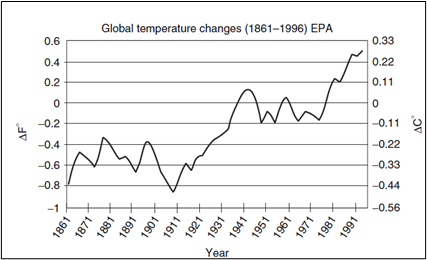
\includegraphics[width=7.5cm]{Figures/My_figures/1-z.png} % Use [width=\linewidth] for full-column figure width
	\caption{Global temperature changes over the years [2]}
	\label{fig:sample}
\end{figure}

Fuel cell vehicles are potentially more efficient and cleaner than internal combustion engines. In this research paper, the main focus is on analysing the behaviour of hybrid vehicles powered by a battery and a hydrogen PEMFC. A stack of fuel cells is first combined with a controller and a computer to understand the performance of the system. The accrued knowledge is then used to define the performance of a hybrid car powered with a battery and a hydrogen PEMFC. [2] [1] [4]
 
Fuel cells are energy converters that transform the chemical energy of a fuel into electrical and thermal energy. The cells’ potential efficiency is high when compared to the combustion engine and the energy density values of their fuels are higher than those of batteries. Each individual fuel cell consists of a bipolar plate (BPP) with an anode and a cathode side, along with a membrane electrode assembly (MEA). The number of individual cells defines the total voltage level, and their active surface area determines current. A PEM fuel cell operates by inducting hydrogen into the anode, where it is oxidized into electrons and protons as per the below equation:

\[H_2 \rightarrow 2H^+ +2e^-,E^{02}=0V\]

The two electrons are not membrane permeable; hence, they travel through the anode electrical interconnect to the load-generating electricity. From there, the electrons travel to the cathode, where they react with the supplied oxygen and the protons that permeate through the membrane to the cathode to form water in a reduction reaction. This process is exothermic.[3]

At the cathode, the reaction is as below:
\[\frac{1}{2} O_2+2e^-+2H^+ \rightarrow H_2 O(l)+Heat,E^01=1.229V\]

Therefore, the overall reaction is as below:

\[H_2+  \frac{1}{2} O_2 \rightarrow H_2 O(l)+Heat,E^0=E^{01}-E^{02}=1.229V\]

\begin{figure}[h] % Single column figure
        \centering
	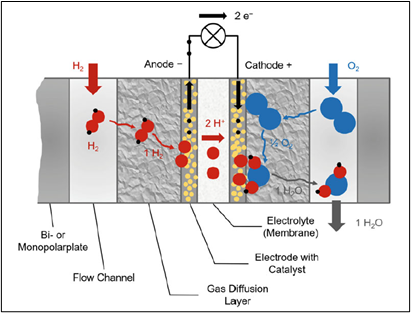
\includegraphics[width=7.5cm]{Figures/My_figures/2-z.png} % Use [width=\linewidth] for full-column figure width
	\caption{Principle of the fuel cell PEMFC [3]}
	\label{fig:sample}
\end{figure}

%------------------------------------------------

\section{Experimental Set Up}

The fuel cell utilised in the first experiment is a stack of 13 fuel cells with a rated voltage and current as 7.8V and 3A respectively. The fuel cell is coupled with fan to catalyse the redox reaction by increasing the oxygen supply into the fuel cell and simultaneously cool the cell down to a target temperature of 35°C. It is equipped with a purge valve to withdraw the water produced as a byproduct of the chemical reaction. The applied load range is 0-3A and is operated by the user through a knob in the control box. Various results are obtained by observing the changes in outputs such as cell voltage, cell temperature, H2 consumption and power. [5]

\begin{figure}[h] % Single column figure
        \centering
	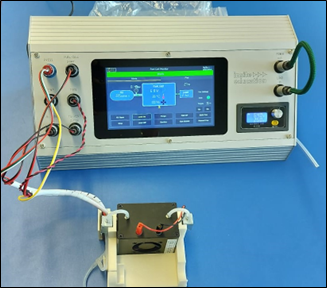
\includegraphics[width=7.5cm]{Figures/My_figures/4-z.png} % Use [width=\linewidth] for full-column figure width
	\caption{H2 engineering kit}
	\label{fig:sample}
\end{figure}

 The second experiment is performed on the FCAT set. It is an integrated miniaturised remote-controlled car. It consists of a comprehensive hybrid propulsion system involving a battery and a HFC to meet the energy needs of the motor driving the wheels. The trainer is mounted on a roller test bench and is connected to a computer for data acquisition. Various conditions of driving were simulated using the FCAT and the observations with graphical interpretations are discussed.
\begin{figure}[h] % Single column figure
        \centering
	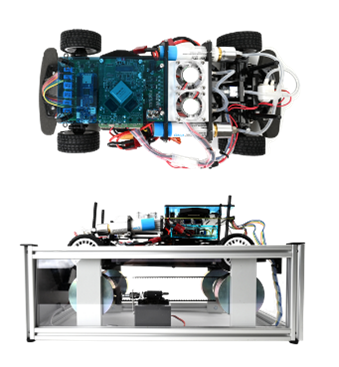
\includegraphics[width=7.5cm]{Figures/My_figures/FCAT comb.png} % Use [width=\linewidth] for full-column figure width
	\caption{FCAT set-up in test bench [14]}
	\label{fig:sample}
\end{figure}

Fuel cells and batteries are both energy sources with their difference in load response respectively, but battery alone takes more charging time than refuelling hydrogen tank. [13]. To overcome both the dis-advantages of fuel cell and the battery Fuel Cell Hybrid Electric Vehicles are emerging as a prominent solution, offering the combined advantages of both the technologies.

\begin{figure}[h] % Single column figure
        \centering
	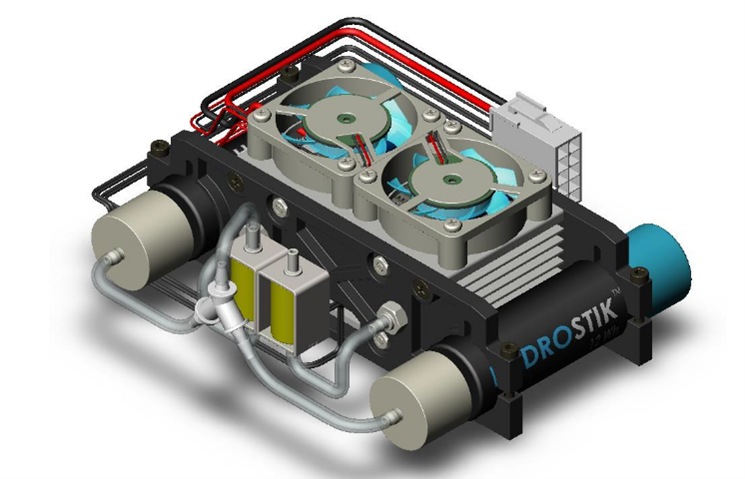
\includegraphics[width=7.5cm]{Figures/My_figures/Hydrogen fuel cell in FCAT.png} % Use [width=\linewidth] for full-column figure width
	\caption{Hydrogen fuel cell in FCAT [14]}
	\label{fig:sample}
\end{figure}

Hybrid vehicles running on a combination of HFC and a battery can be a synthesis of two different kinds of sustainable energy working together to create a far more efficient system. Although, the function of an energy management system is crucial. It controls the energy splitting between two energy sources.

\begin{figure}[h] % Single column figure
        \centering
	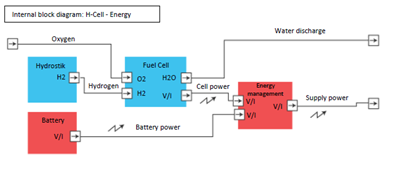
\includegraphics[width=7.5cm]{Figures/My_figures/EMS.png} % Use [width=\linewidth] for full-column figure width
	\caption{Block diagram of hybrid propulsion system [15]}
	\label{fig:sample}
\end{figure}

Through the utilisation of FCAT in various simulated situations, the performance of the FCAT has been understood and plotted as graphs in the next section.   

%------------------------------------------------

\section{Experimental Results and Observations of Hydrogen PEMFC with Engineering Kit}


The characteristics of the fuel cell are analyzed by varying the current in step-wise increments of 0.3 A per step.

In this experiment, the fuel cell stack used has total 13 cells arranged in series to form a one single stack.
The characteristic curves of the fuel cell are influenced by the hydrogen consumption (ml/min), pressure of hydrogen (mBar), fan speed (\%), purge process, power (W), cell temperature (°C), cell voltage (V), and load current (A) of the fuel cell membranes. The detailed behavioural characteristics of the fuel cell are described below.
\textbf{\subsection{Voltage Current Characteristics}}
The voltage-current curve of the fuel cell is as shown Figure-7. The external load of current has been supplied to the fuel cell. Therefore, to overcome the load current the maximum emf has been produced from the hydrogen -oxygen collision at the cathode. 
\begin{figure}[h] % Single column figure
        \centering
	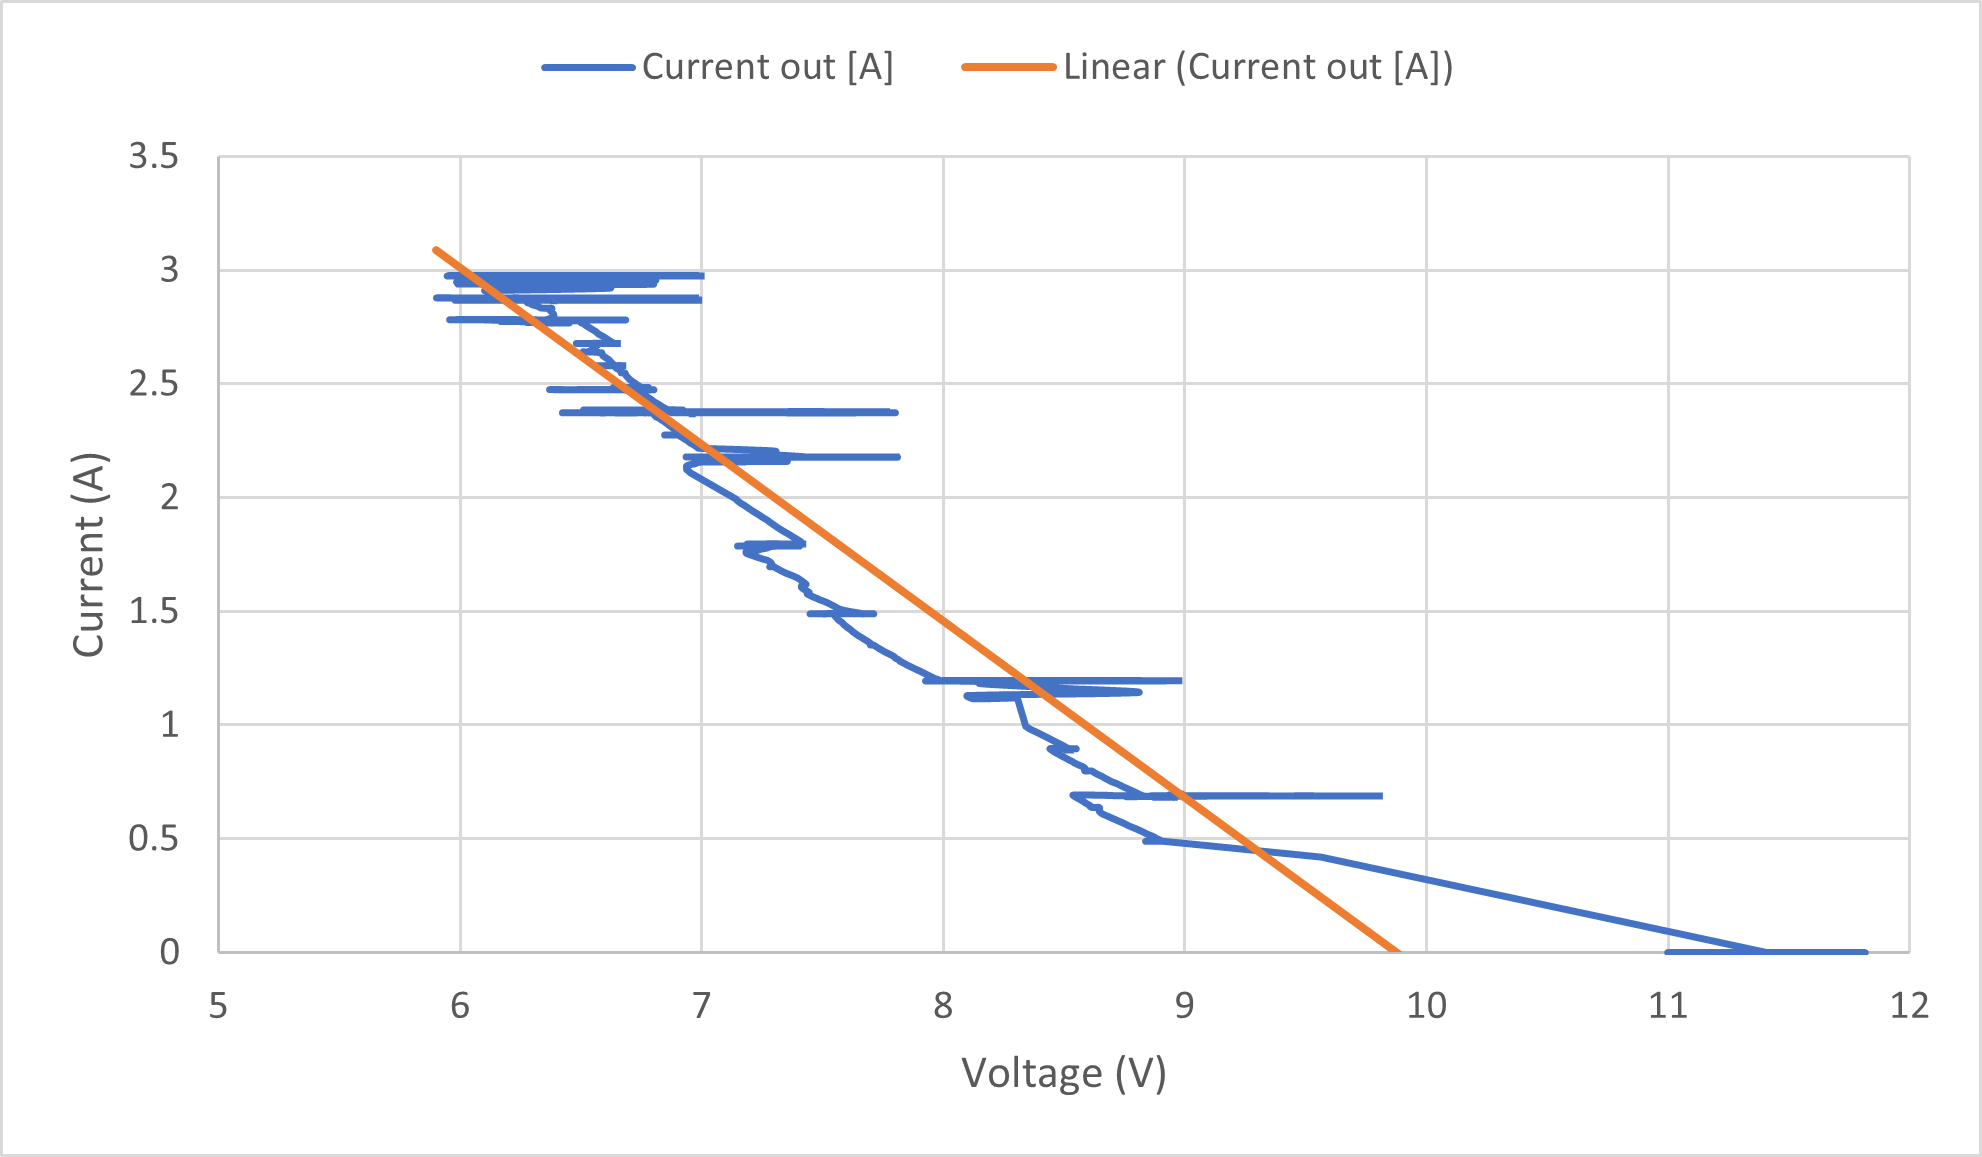
\includegraphics[width=7.5cm;]{Figures/My_figures/VI curve.png} % Use [width=\linewidth] for full-column figure width
	\caption{Voltage-current characteristics}
	\label{fig:sample}
\end{figure}
The produced voltage and supplied current follows a linear relationship and are inversely proportional to each other. The major observation from the V-I curve is that the voltage decreases as the current increases.
\begin{figure}[h] % Single column figure
        \centering
	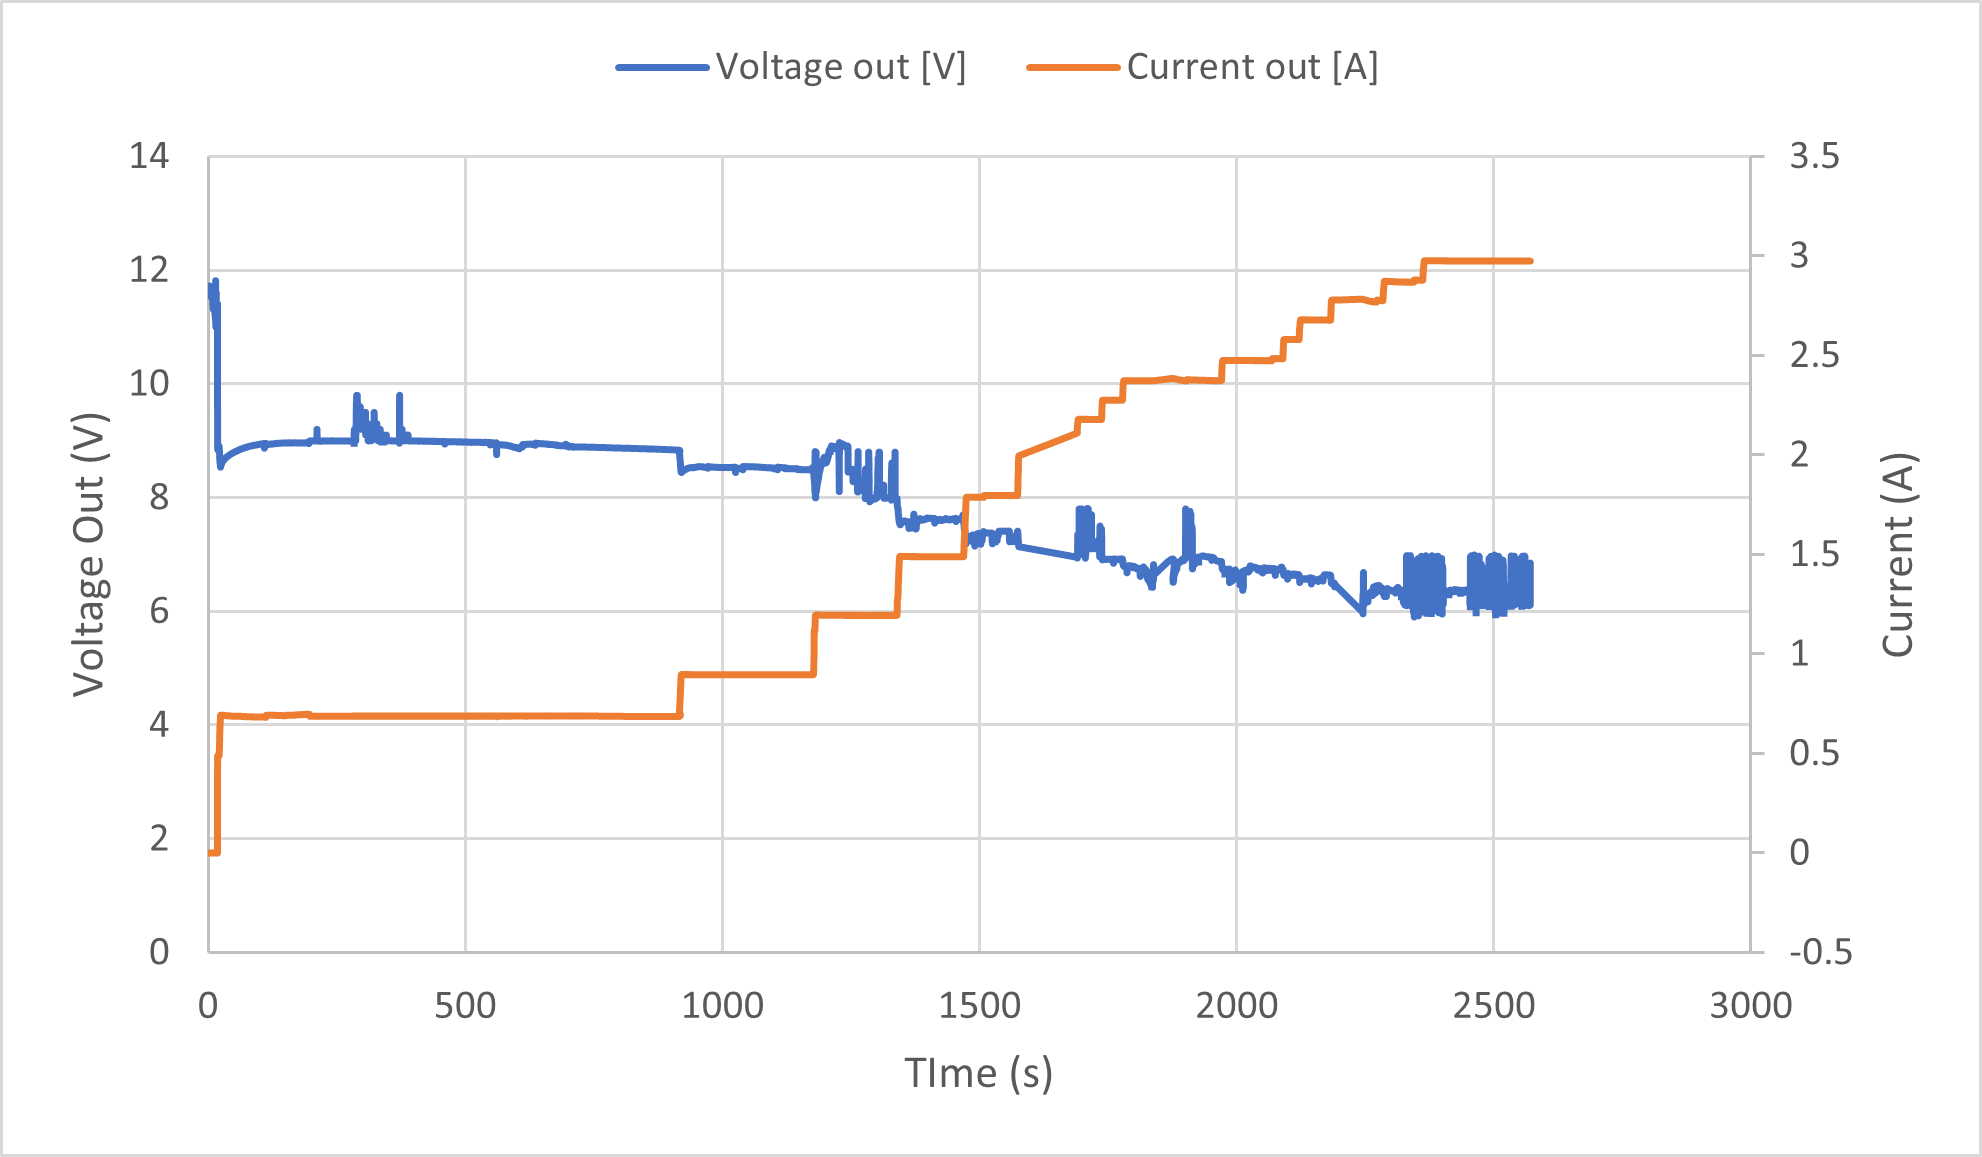
\includegraphics[width=7.5cm;]{Figures/My_figures/VI_with time.png} % Use [width=\linewidth] for full-column figure width
	\caption{Voltage-current characteristics with respect to time}
	\label{fig:sample}
\end{figure}
Figure-9 depicts the inverse relationship between current and voltage. During initial phase, voltage decreases rapidly as the current increases, then as the current remains constant, the voltage also remains constant, followed by a final gradual increase in current and decrease in voltage. 
\textbf{\subsection{Hydrogen Consumption-Current Characteristics}}
The characteristic curve of the hydrogen consumption of the fuel cell with the change in current is as shown in Figure-9. The hydrogen consumption increases as the current increases on the fuel cell that the demand on the cell increased to generate maximum output. Interestingly, the pattern of both the curves are very identical indicating that the demand placed on the hydrogen cell is instantaneously met with the hydrogen supply.
\begin{figure}[h] % Single column figure
        \centering
	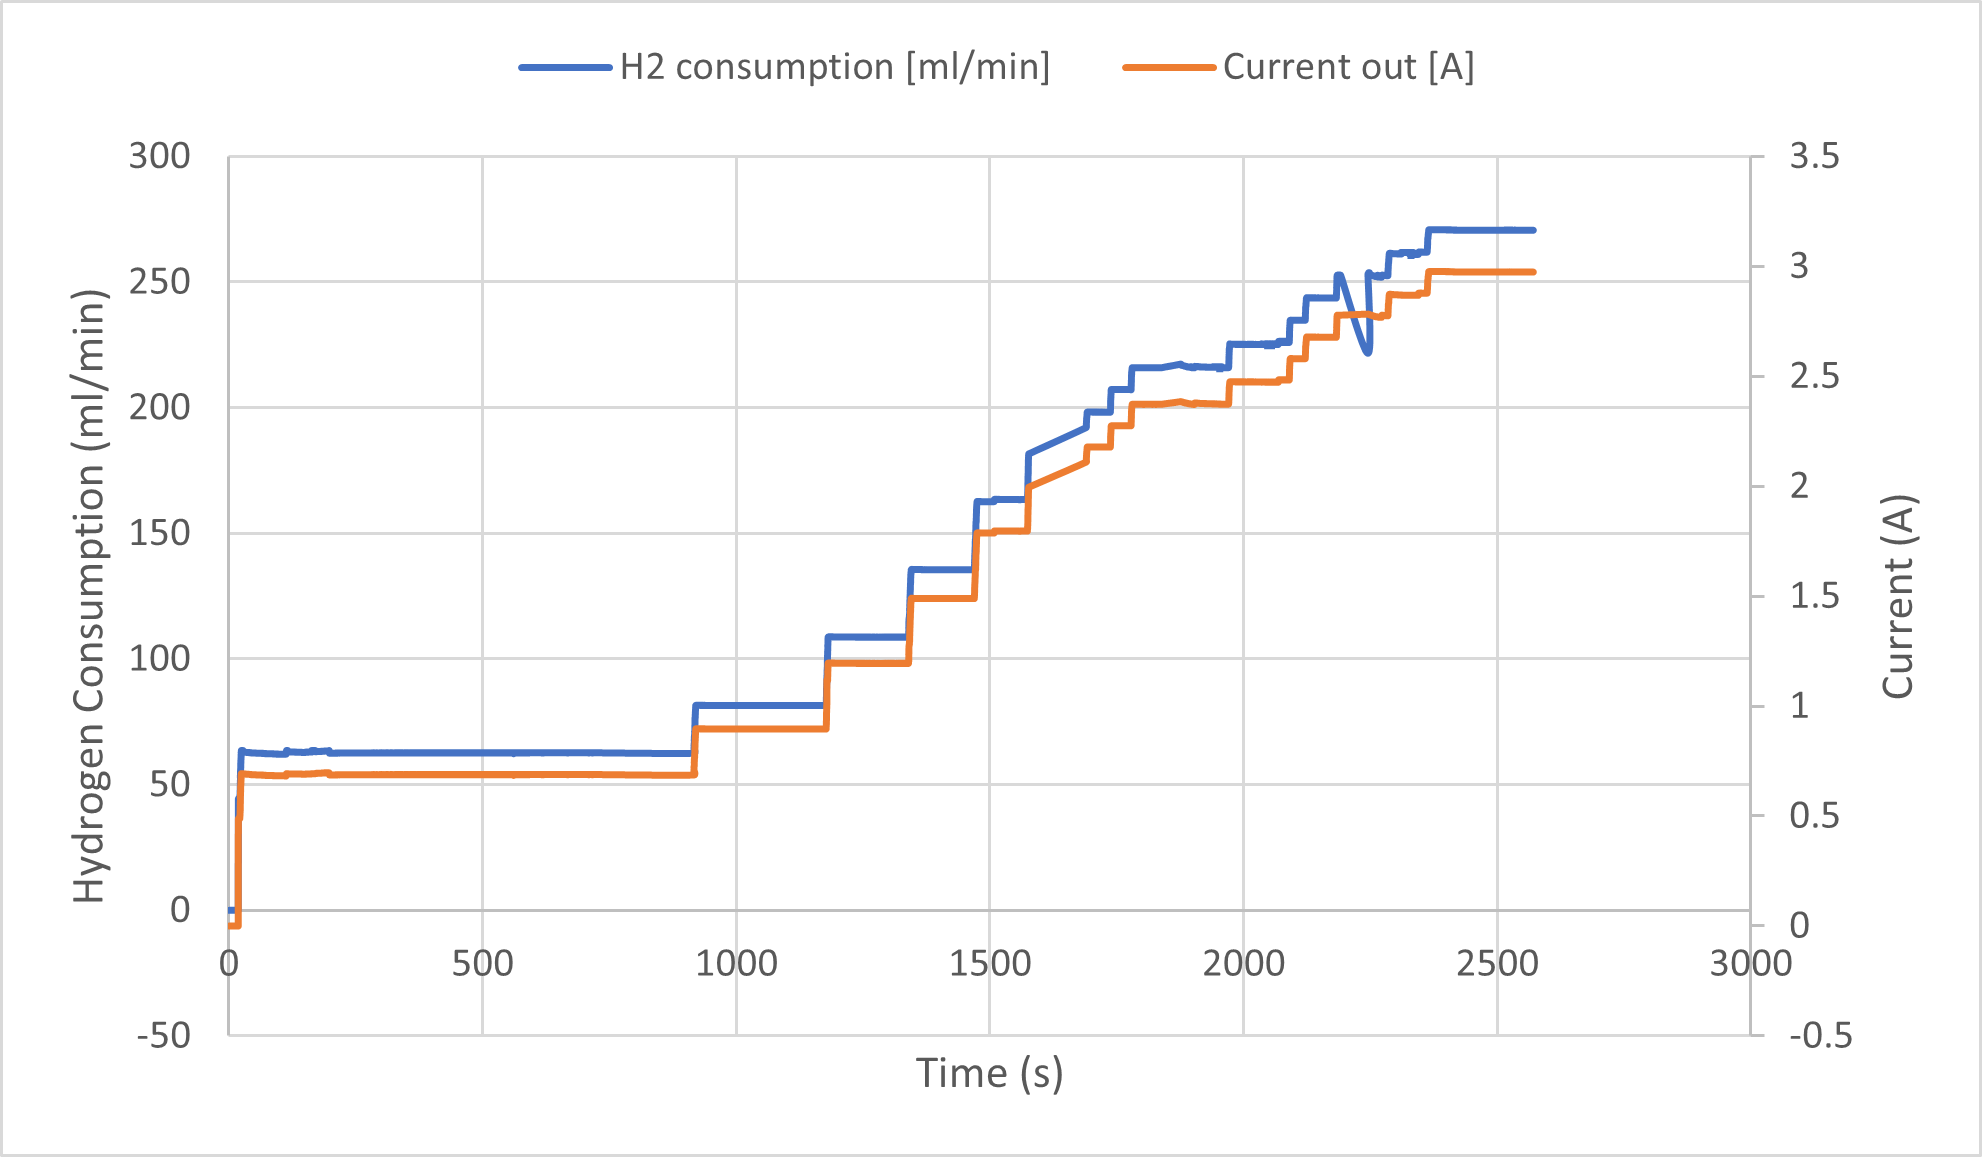
\includegraphics[width=7.5cm;]{Figures/My_figures/Hydcons_current_time.png} % Use [width=\linewidth] for full-column figure width
	\caption{Hydrogen-current characteristics}
	\label{fig:sample}
\end{figure}
\textbf{\subsection{Power-current characteristics}}
The characteristic curve of the power produced from the fuel cell with respect to the change in current is as shown in Figure-10. Both the power and current follow a linear relationship and are directly proportional to each other. 

\begin{figure}[h] % Single column figure
        \centering
	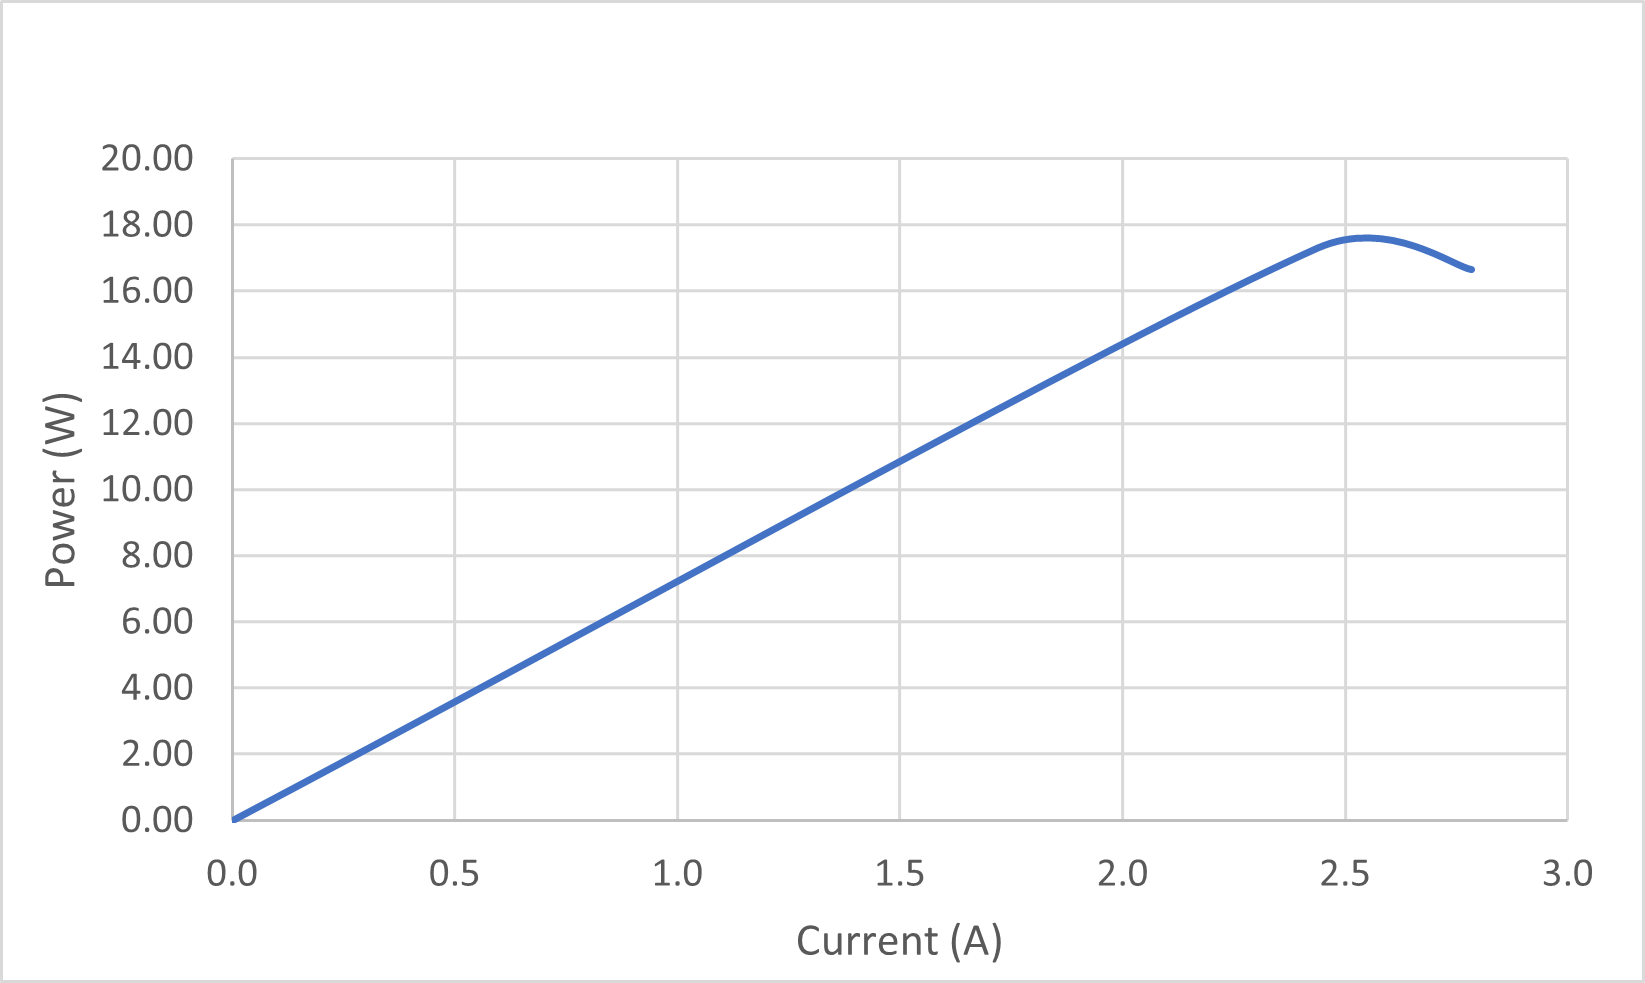
\includegraphics[width=7.5cm;]{Figures/My_figures/Power_current.png} % Use [width=\linewidth] for full-column figure width
	\caption{Power-Current Characteristics}
	\label{fig:sample}
\end{figure}

Nevertheless, beyond a certain threshold value a subsequent decline in power is inevitable [3]. From the current 2.5 A onwards there is a slight decline in the curve from the graph. Hence, it can be concluded the power output of the fuel cell decreases at slightly below the point of maximum load carrying capacity of the fuel cell.
\textbf{\subsection{Fuel Cell Temperature-Current Characteristics}}

 In this section, the study on the effect of cell temperature on the performance of fuel stack is conducted. It mainly depends on the fan speed and the amount of load acting on the cell. The fuel cell is maintained at a constant load of current 3A and and is observed for the changes in voltage by controlling the fan speed, which in turn indirectly controls the cell temperature. Subsequently, a comparative analysis of performance ensues, contrasting the outcomes achieved under higher and lower cell temperatures. Comparative analysis of the performance of voltage-cell temperature under high and low cell temperatures is as shown in Figure-11 and Figure 12.

\begin{figure}[h] % Single column figure
        \centering
	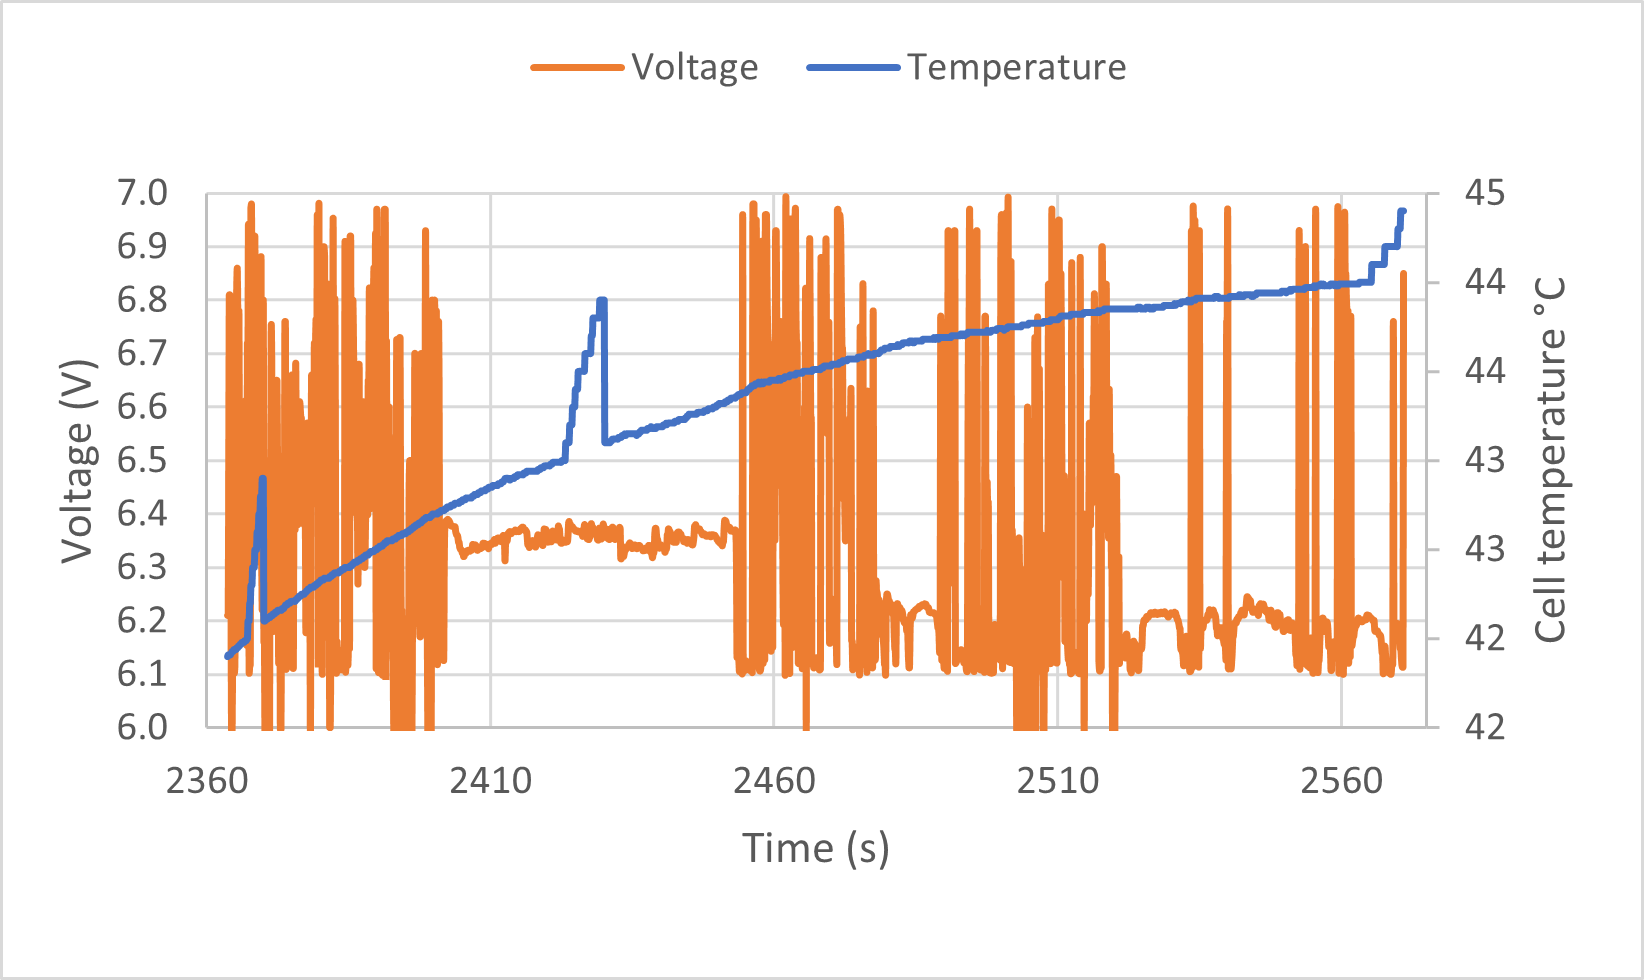
\includegraphics[width=7.5cm;]{Figures/My_figures/High temp cell.png} % Use [width=\linewidth] for full-column figure width
	\caption{Voltage-cell temperature with respect to time at constant current 3 A - high temperature condition}
	\label{fig:sample}
\end{figure}

The range of voltages in Y axis is 6-7V for the high temperature condition and 6.8-8V in the low temperature condition.The high temperature range can be read out from the as 41.5-44.5°C, whereas the low temperature range is 34.5-37°C. This comparison indicates that the voltage level achieved for the same current level is much higher at lower temperatures than at higher temperatures. The minimum voltage level is 0.8V higher in the low temperature condition than the higher temperature condition. The peak value attained is also 1V higher in the low temperature state.

\begin{figure}[h] % Single column figure
        \centering
	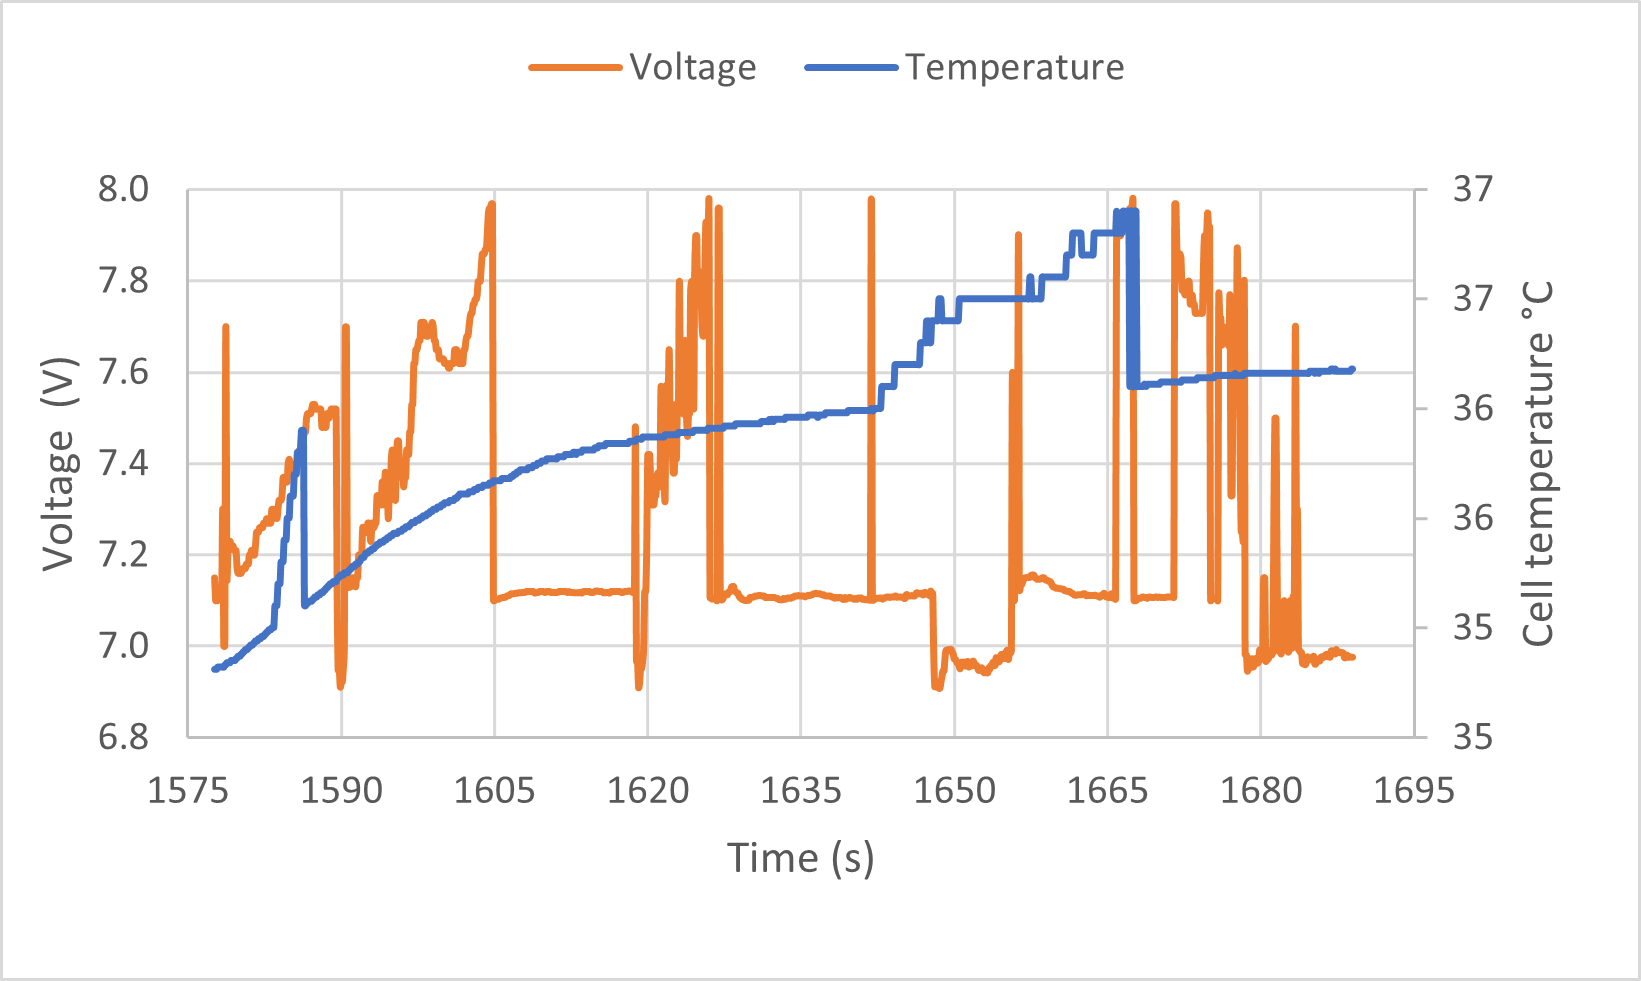
\includegraphics[width=7.5cm;]{Figures/My_figures/low temp cell.png} % Use [width=\linewidth] for full-column figure width
	\caption{Voltage-cell temperature with respect to time at constant current 3 A - low temperature condition}
	\label{fig:sample}
\end{figure}

Typically, thermally-activated processes, such as chemical reactions, exhibit exponential growth in rates with escalating temperatures. Consequently, a logical inference would suggest a substantial increase in the rates of proton transport in the electrolyte and oxygen reduction at the cathode with elevated operating temperatures. However, attaining such results poses challenges due to the simultaneous deterioration of the system’s water balance as the temperature rises. Dehydration of the electrolyte membrane negatively affects proton transport mechanisms, oxygen-reduction kinetics, thereby manifesting in a diminished overall cell performance [8]. Therefore the performance of the cell mainly depends on the cell temperature.

\section{Experimental results and Observations of Hybrid Propulsion System with FCAT}

The Fuel Cell Automotive Trainer (FCAT) is an integrated miniaturised remote-controlled car. It consists of a comprehensive hybrid propulsion system involving a battery and a HFC. The vehicle is mounted on a roller test bench set-up and it is connected to a computer for data acquisition. It collects the data of speed (m/s), battery voltage (V), fuel cell voltage (V), output voltage (V), battery current (A), fuel cell current (A), time (s), output current (A), and braking force (N) under various conditions of driving. The output voltage is the mixture of the battery voltage and the HFC voltage. It is an output of the energy management system. This is also applicable for the output current. The detailed study on the behaviour of currents and voltages characteristics under various driving conditions were simulated with graphical interpretations are discussed below.
\textbf{\subsection{Engine ON-Idle State}}
In the initial condition, when the hybrid engine with the HFC and the battery is started, there is no movement of the vehicle. The HFC and battery start generating the voltage according to its capacity. The voltage curves of the HFC and the battery can be observed from Figure 13. It is apparent that the voltage of the hydrogen cell is the highest at approximately 10V, whereas the battery voltage and output voltage are maintained at 8V. HFC starts to produce emf in smaller range at first and then gradually increases the voltage to the maximum capacity. 

\begin{figure}[h] % Single column figure
        \centering
	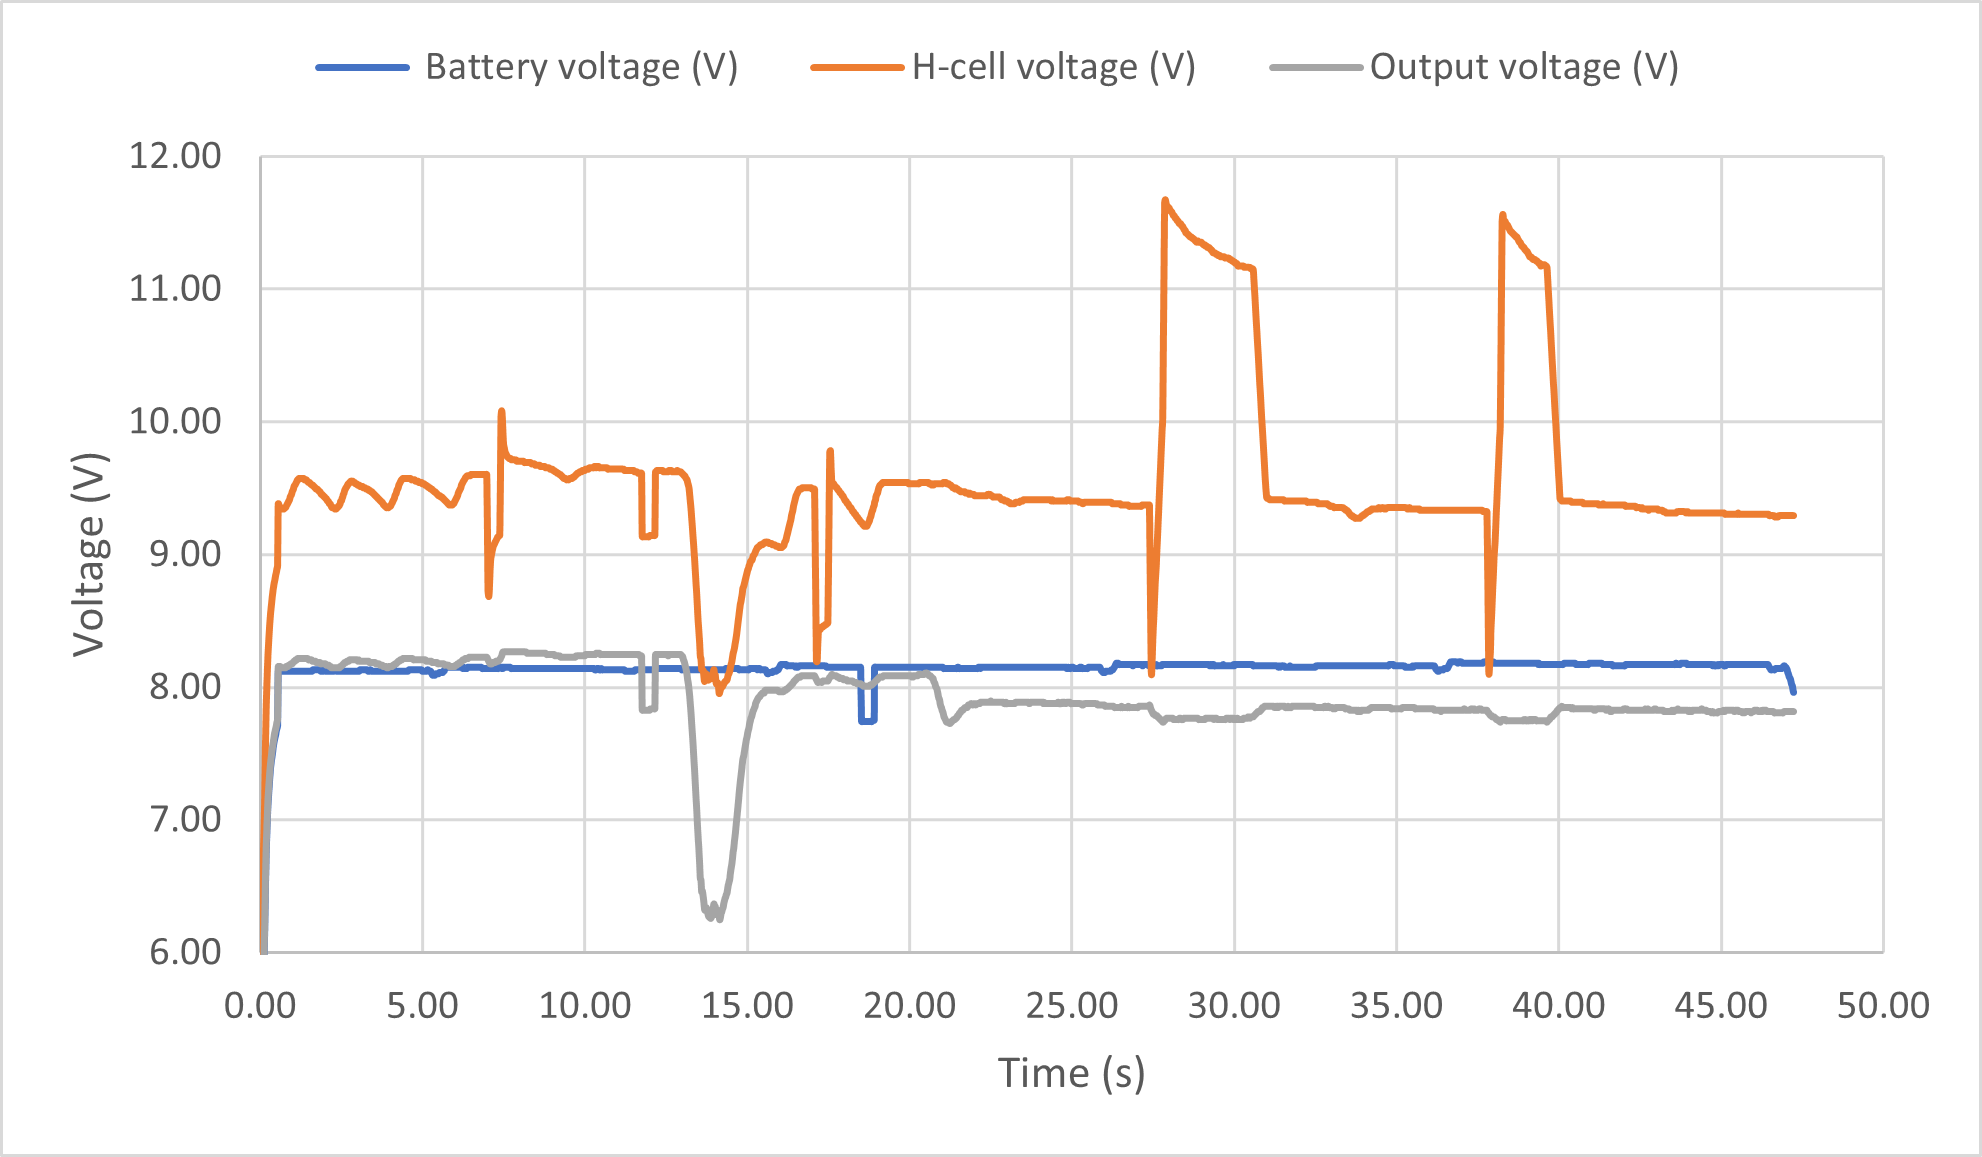
\includegraphics[width=7.5cm;]{Figures/My_figures/All Voltages vs time.png} % Use [width=\linewidth] for full-column figure width
	\caption{Characteristics of voltages in engine ON idle state}
	\label{fig:sample}
\end{figure}

The characteristic curves of the battery current, HFC current and output current with respect to time in idle condition is as shown in Figure-14. The output current is a little over the 0-line indicating that the net load is 0 because of the idling condition. \begin{figure}[h] % Single column figure
        \centering
	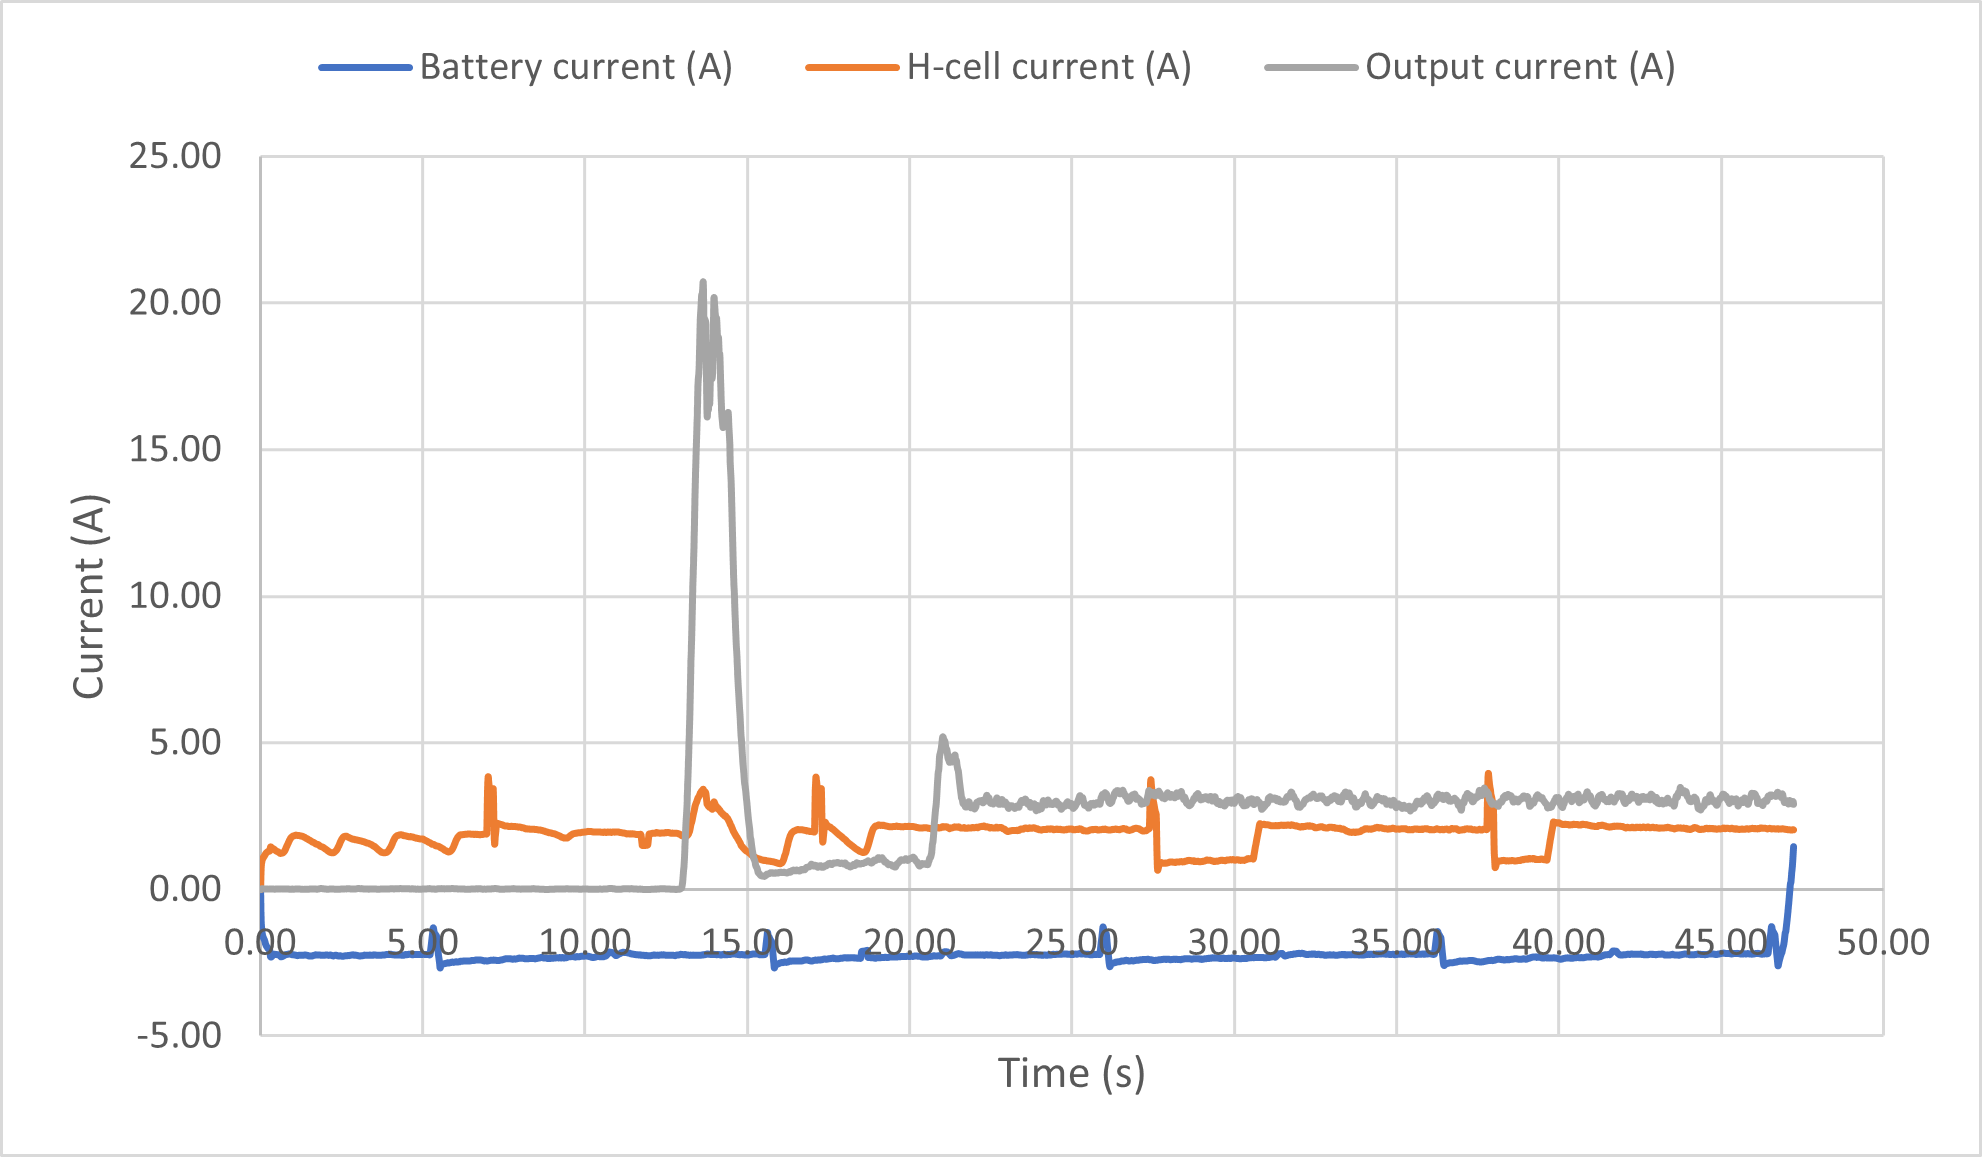
\includegraphics[width=7.5cm;]{Figures/My_figures/All currents vs time.png} % Use [width=\linewidth] for full-column figure width
	\caption{Characteristics of current in engine ON idle state}
	\label{fig:sample}
\end{figure}
It has been observed that the battery current is in the negative area, indicating that the battery is getting re-charged from the power produced by the HFC. The HFC current line indicates that the load is due to charging of the battery in the idle condition. From the graph, it can be observed that  current of the battery remains negative indicating that whenever the vehicle is in a no-load condition, the battery tends to shift to being in a charging state by the HFC. 
\textbf{\subsection{Gradual Acceleration}}

To understand the complete behaviour of the hybrid powered model car, it is essential to understand its performance when accelerating gradually. The current and voltage characteristics of the system against time during gradual acceleration from 0 to 8 m/s is shown in Figures 15 and 16. The battery current switches from the negative to  positive as the speed increases from 0 to maximum. 
\begin{figure}[h] % Single column figure
        \centering
	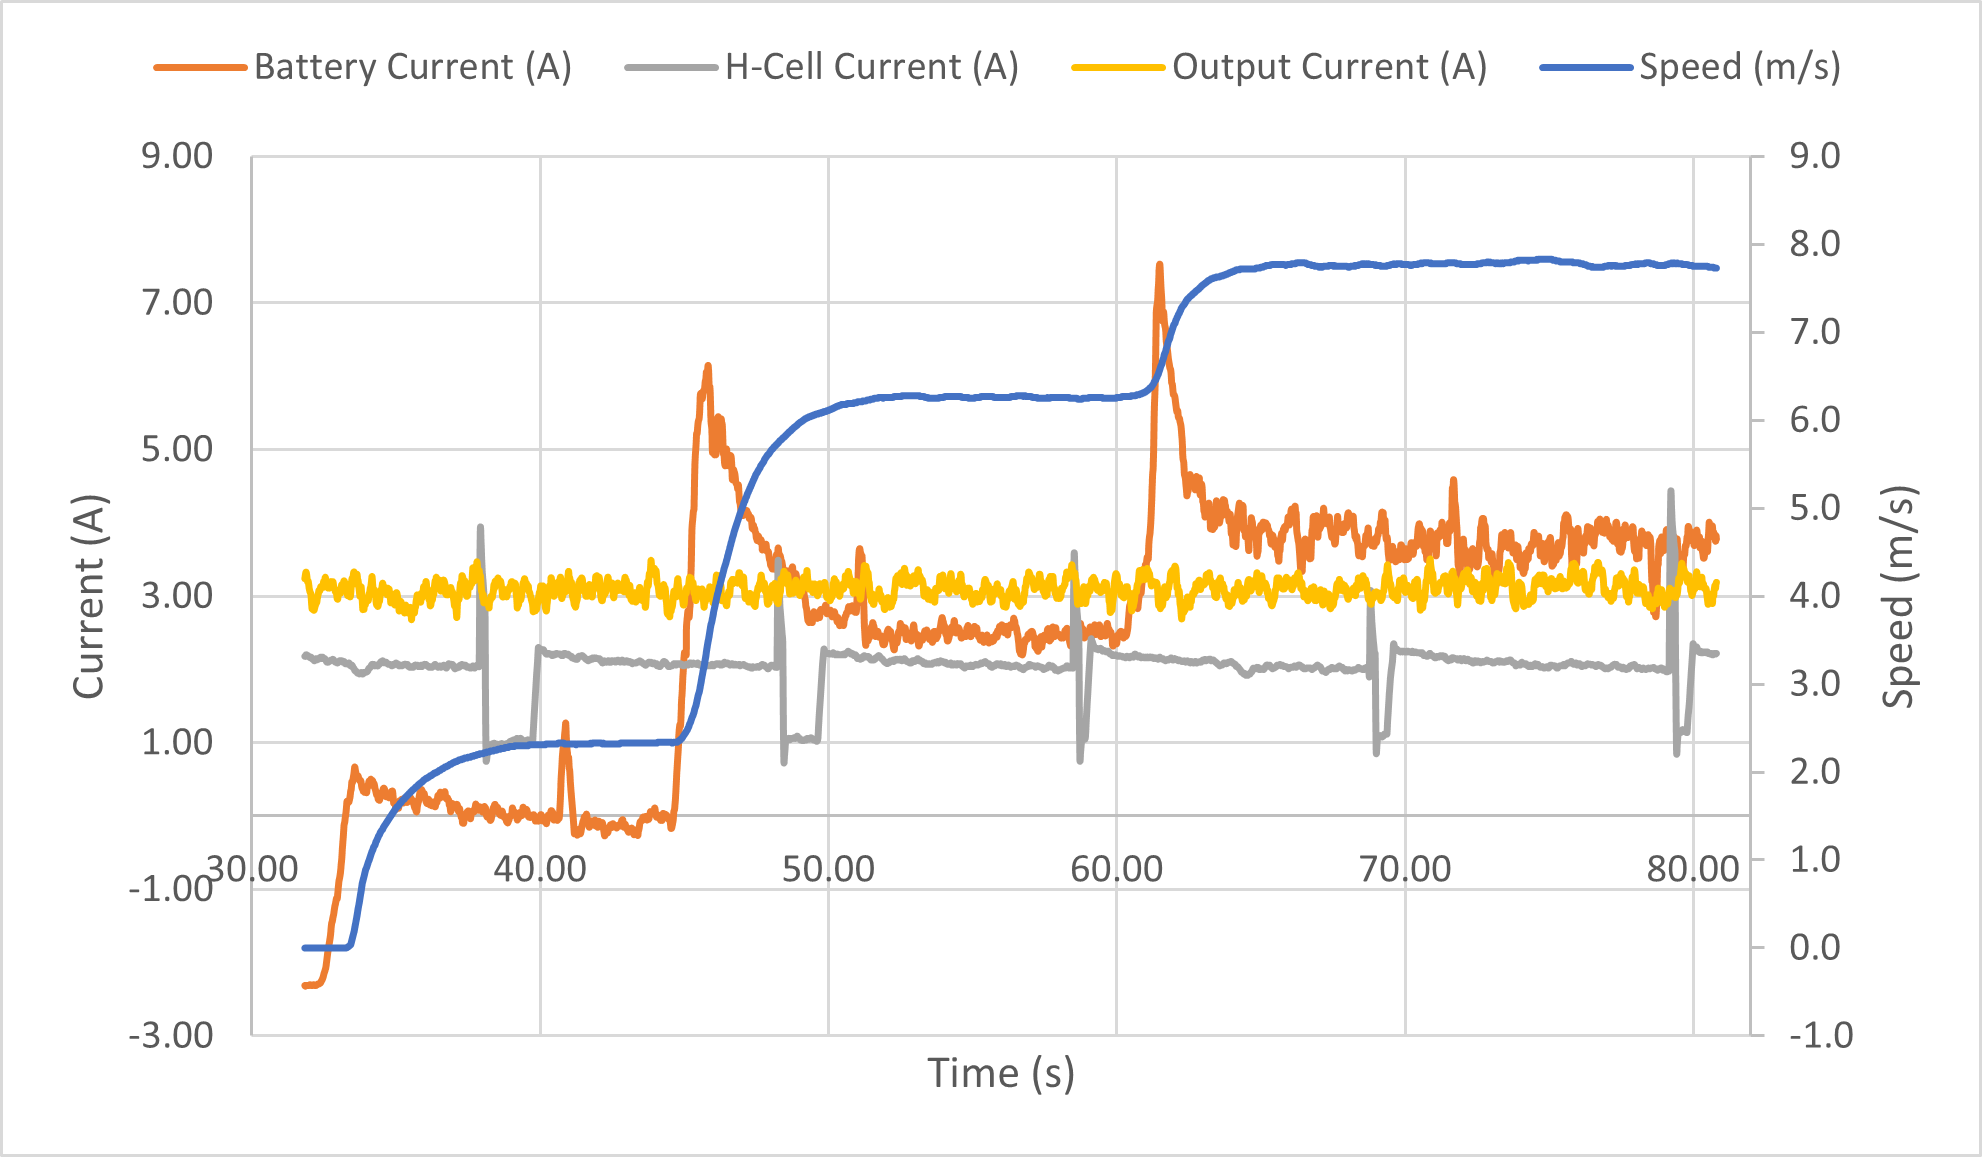
\includegraphics[width=7.5cm;]{Figures/My_figures/case1-All Currents vs Time.png} % Use [width=\linewidth] for full-column figure width
	\caption{Current characteristics during gradually acceleration}
	\label{fig:sample}
\end{figure}
For every change in speed there is a change in the battery current also, that means the battery is the affected part with the increase in speed of the vehicle. On the other hand, the output current is maintained constant by the energy management system. When the speed and the corresponding load suddenly increase, the battery current increases, whereas the HFC is maintained in a steady-state condition. In some cases, when the battery current decreases, the HFC plays a pivotal role in compensating for the load acting on the vehicle. 

\begin{figure}[h] % Single column figure
        \centering
	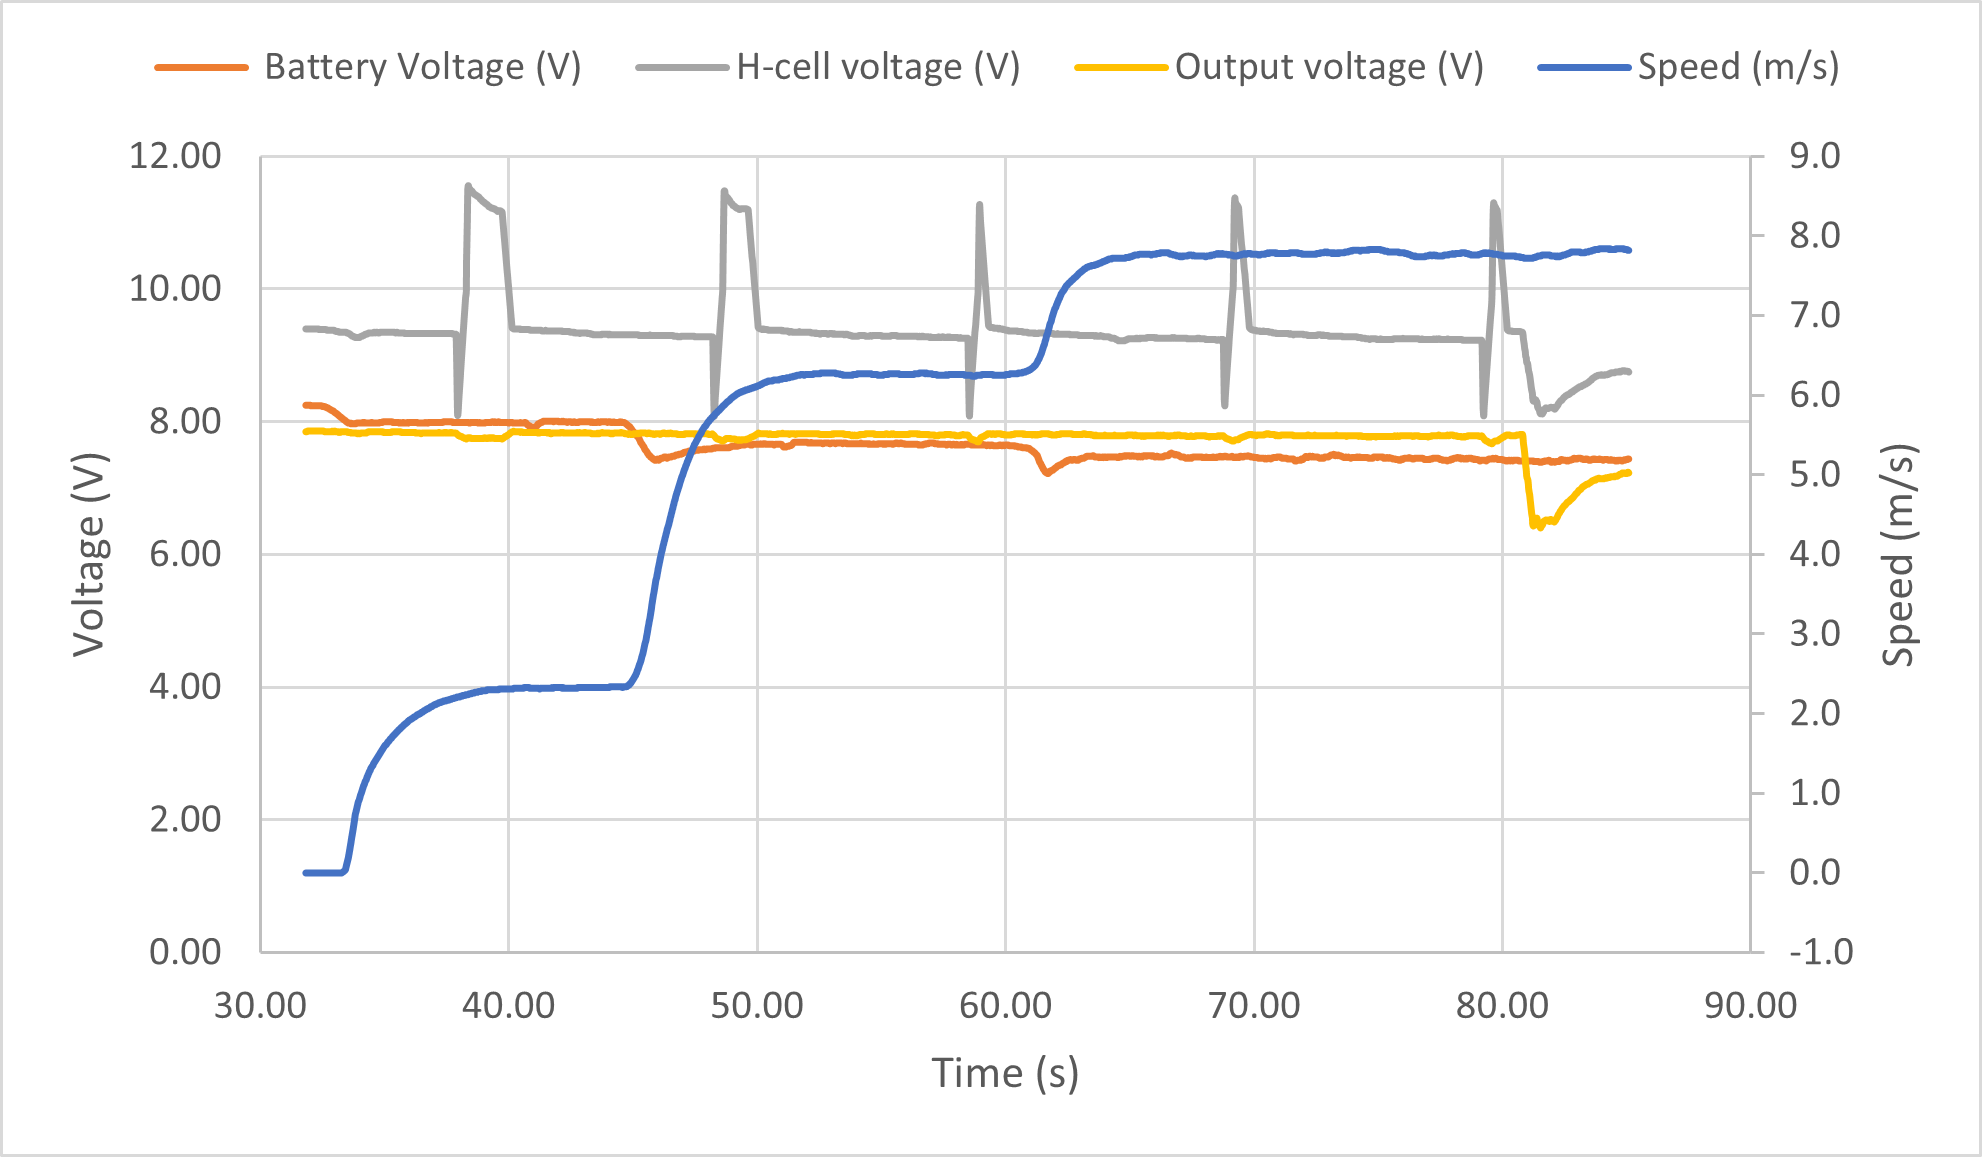
\includegraphics[width=7.5cm;]{Figures/My_figures/case1-All Voltages vs Time.png} % Use [width=\linewidth] for full-column figure width
	\caption{Voltage characteristics in during gradually acceleration}
	\label{fig:sample}
\end{figure}

Voltage characteristics of the fuel cell and battery with respect to the time with the change in speed is as shown in the Figure-16. From the current characteristic curve of the same loading condition, it is observed that there is a change in the battery current. 
Consequently, for the same loading condition the battery voltage decreases for each increment in speed. 
The change in magnitude of the voltage during gradual acceleration is in the range of 2 – 2.5 V for both the battery and HFC sources, Whereas the output voltage remains constant in order to compensate total load acting on the vehicle.
\textbf{\subsection{Rapid Acceleration}}

In this condition, vehicle tends to increase its speed rapidly to its maximum limit in a short duration. The characteristic curves of battery current and HFC current have been plotted with respect to speed in the time interval is as shown in Figure-17. It is noticeable that the battery current significantly increases, whereas the HFC current remains constant as the speed increases rapidly. This indicates that the energy demand during rapid acceleration is placed on the battery by the energy management system. At the initial stage, the battery current increases proportionally to the speed.

\begin{figure}[h] % Single column figure
        \centering
	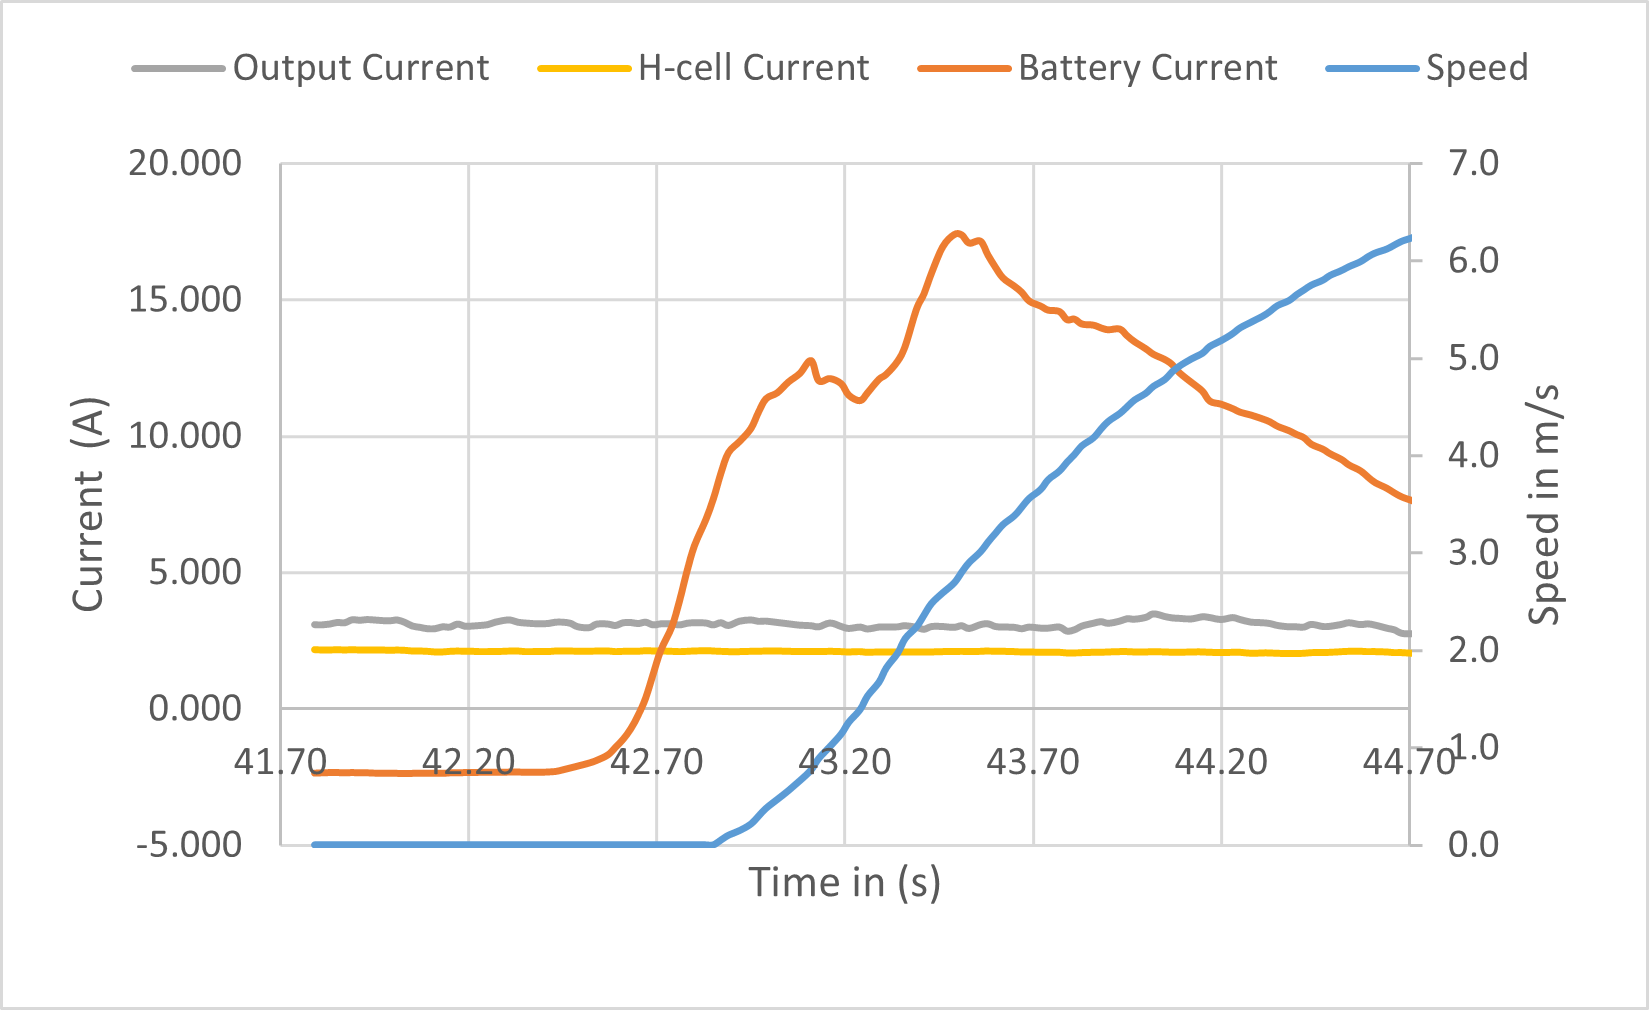
\includegraphics[width=7.5cm;]{Figures/My_figures/CASE-3 All current vs time.png} % Use [width=\linewidth] for full-column figure width
	\caption{Current characteristics in rapid increased speed}
	\label{fig:sample}
\end{figure}
The voltages of the HFC and battery is as shown in the Figure-18. With the change in current from the battery there is a change in voltage. The battery voltage and current exhibit an inversely proportional relationship with each other. In this scenario of rapid acceleration, energy is to be spent to drive the vehicle at the required speed. This phase of rapid acceleration is supported by the battery voltage, after which the current reduces when the vehicle is driven at a constant speed. And it is apparent in this case that as the speed increases rapidly, the battery voltage decreases simultaneously indicating that the voltage from the battery is used to drive the wheels. On the other hand, the HFC voltage increases which signifies that the energy management system triggers the HFC to produce more voltage by inducing the redox reaction. Once the saturation point is attained, the battery voltage is observed to slightly increase in its value, indicating that the battery is being recharged by the HFC as the energy demand placed on the energy management system has reduced.
\begin{figure}[h] % Single column figure
        \centering
	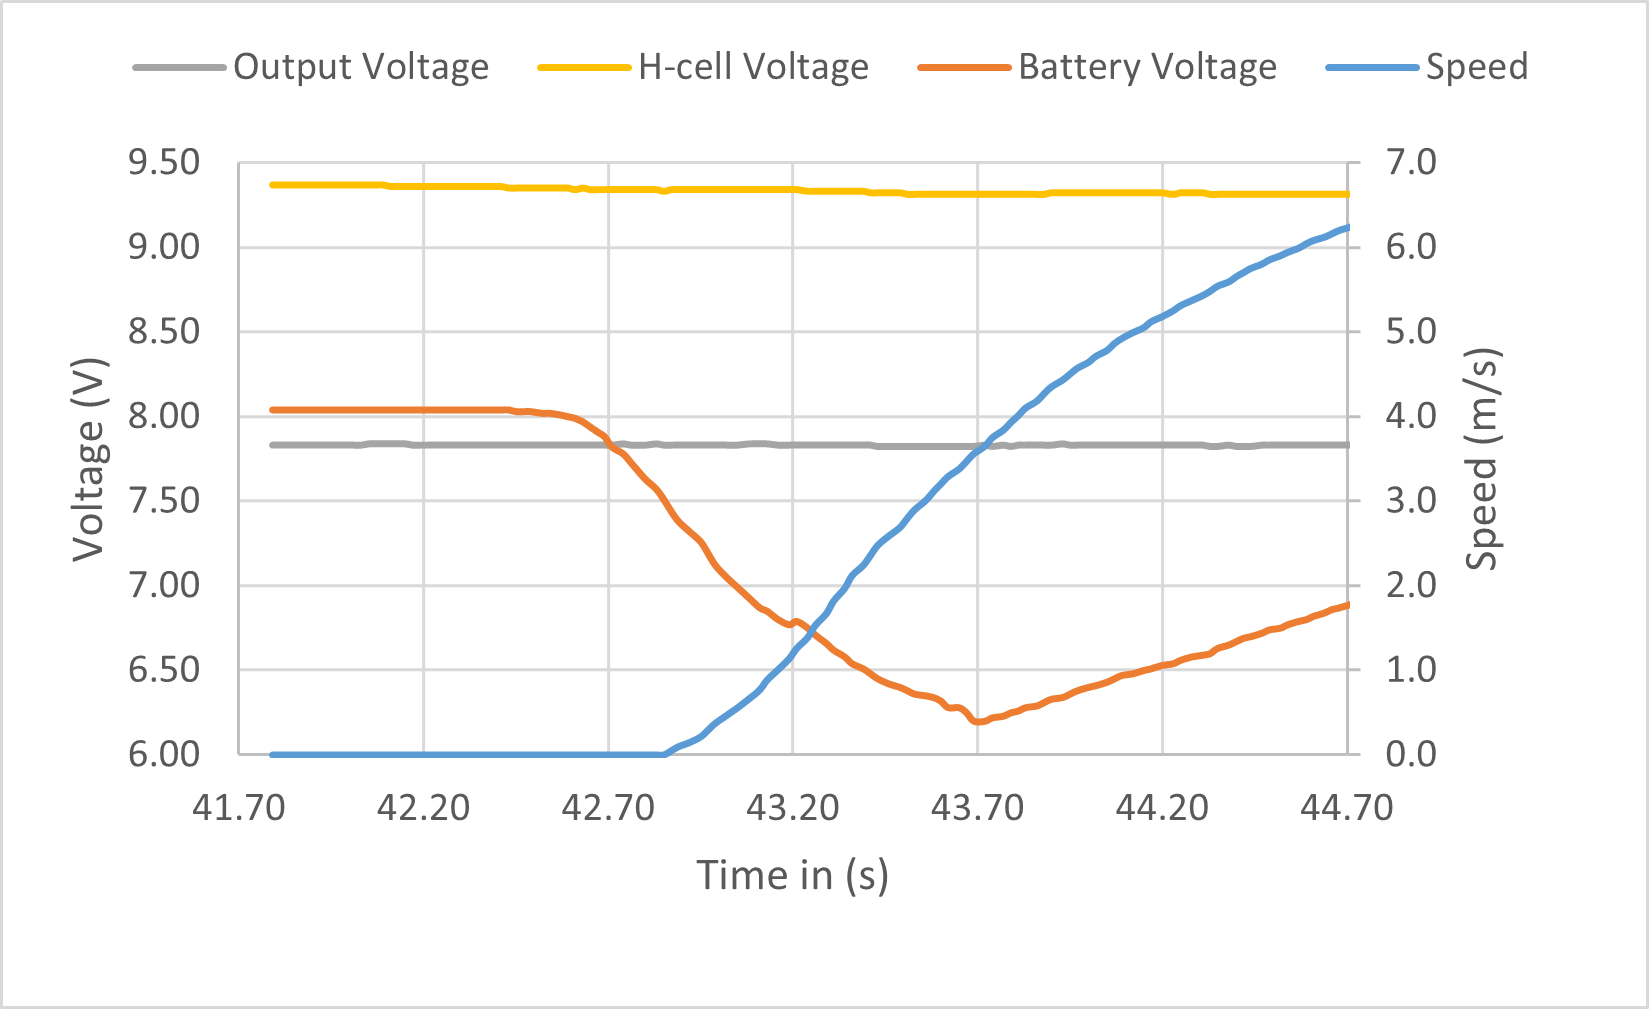
\includegraphics[width=7.5cm;]{Figures/My_figures/CASE-3 All voltages vs time.png} % Use [width=\linewidth] for full-column figure width
	\caption{Voltage characteristics during rapid acceleration}
	\label{fig:sample}
\end{figure}
\textbf{\subsection{Constant Speed}}

The characteristics curves of the various currents of the hybrid car when driving at a constant speed at 2 m/s and 6 m/s are analysed and depicted below in Figures 19 and 20. The short and small dips in the battery and HFC curves indicate that the energy required to drive the vehicle at this speed is minuscule. At lesser constant speed, the HFC current is more than the battery current. This means that the energy required for driving the wheels is majorly supplied from the HFC.

\begin{figure}[h] % Single column figure
        \centering
	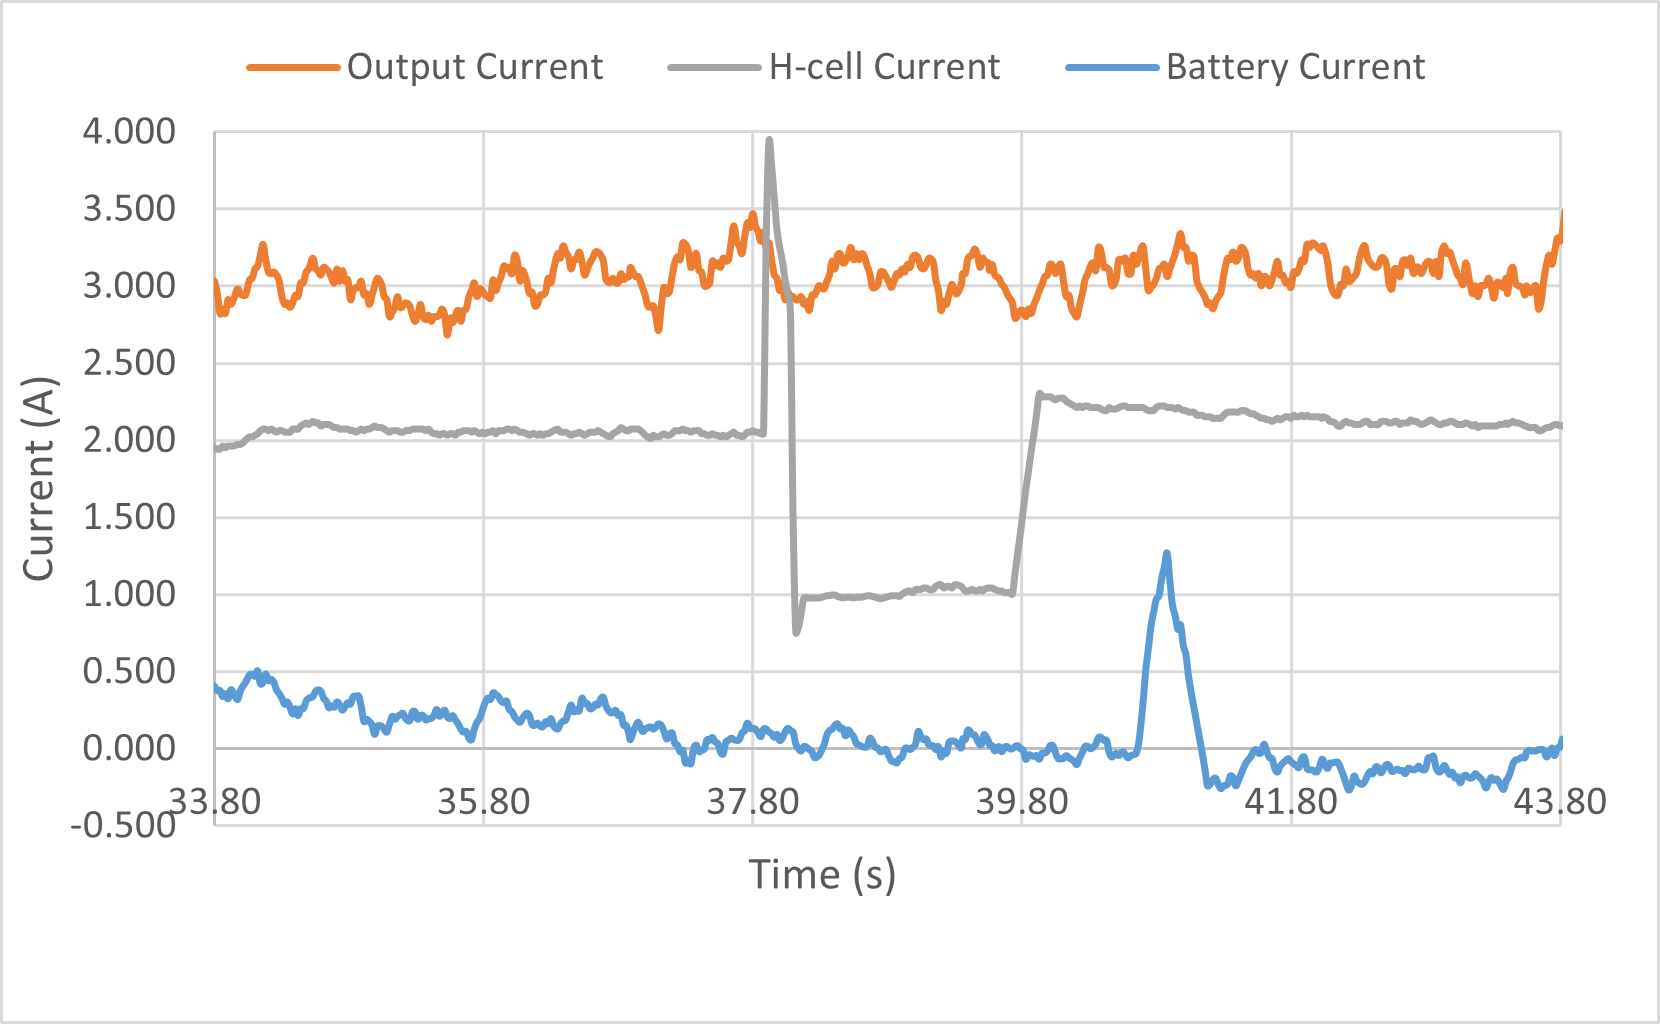
\includegraphics[width=7.5cm;]{Figures/My_figures/CASE-4 All currents vs time 2ms.png} % Use [width=\linewidth] for full-column figure width
	\caption{Current characteristics at constant speed 2 m/s}
	\label{fig:sample}
\end{figure}

The battery current curve signifies a downward trend and moves decisively into the charging state after 6 seconds of constant speed driving. The HFC continues to drive the wheels. 
\begin{figure}[h] % Single column figure
        \centering
	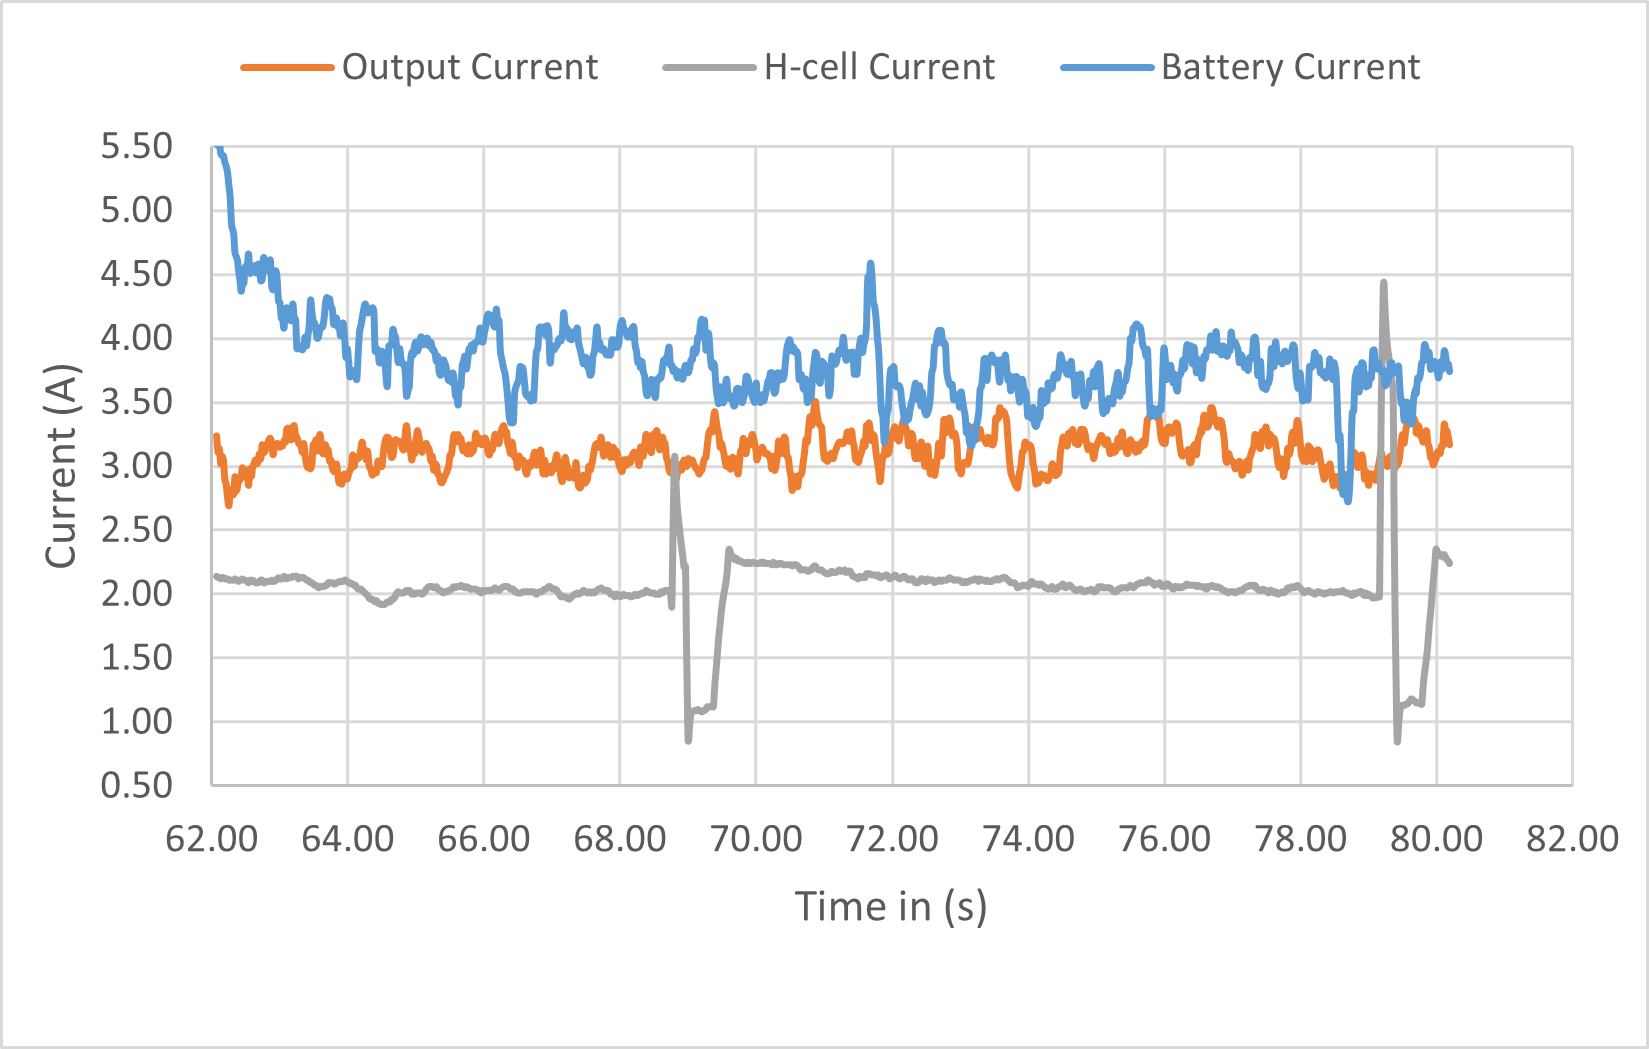
\includegraphics[width=7.5cm;]{Figures/My_figures/CASE-4 All currents vs time.png} % Use [width=\linewidth] for full-column figure width
	\caption{Current characteristics at constant Speed 6 m/s}
	\label{fig:sample}
\end{figure}
The increase in speed  to 6 m/s increases the battery current more than the HFC current. In this case, the increased speed load has been shared by the battery. The output current remained constant through all the changes in speed. 

\begin{figure}[h] % Single column figure
        \centering
	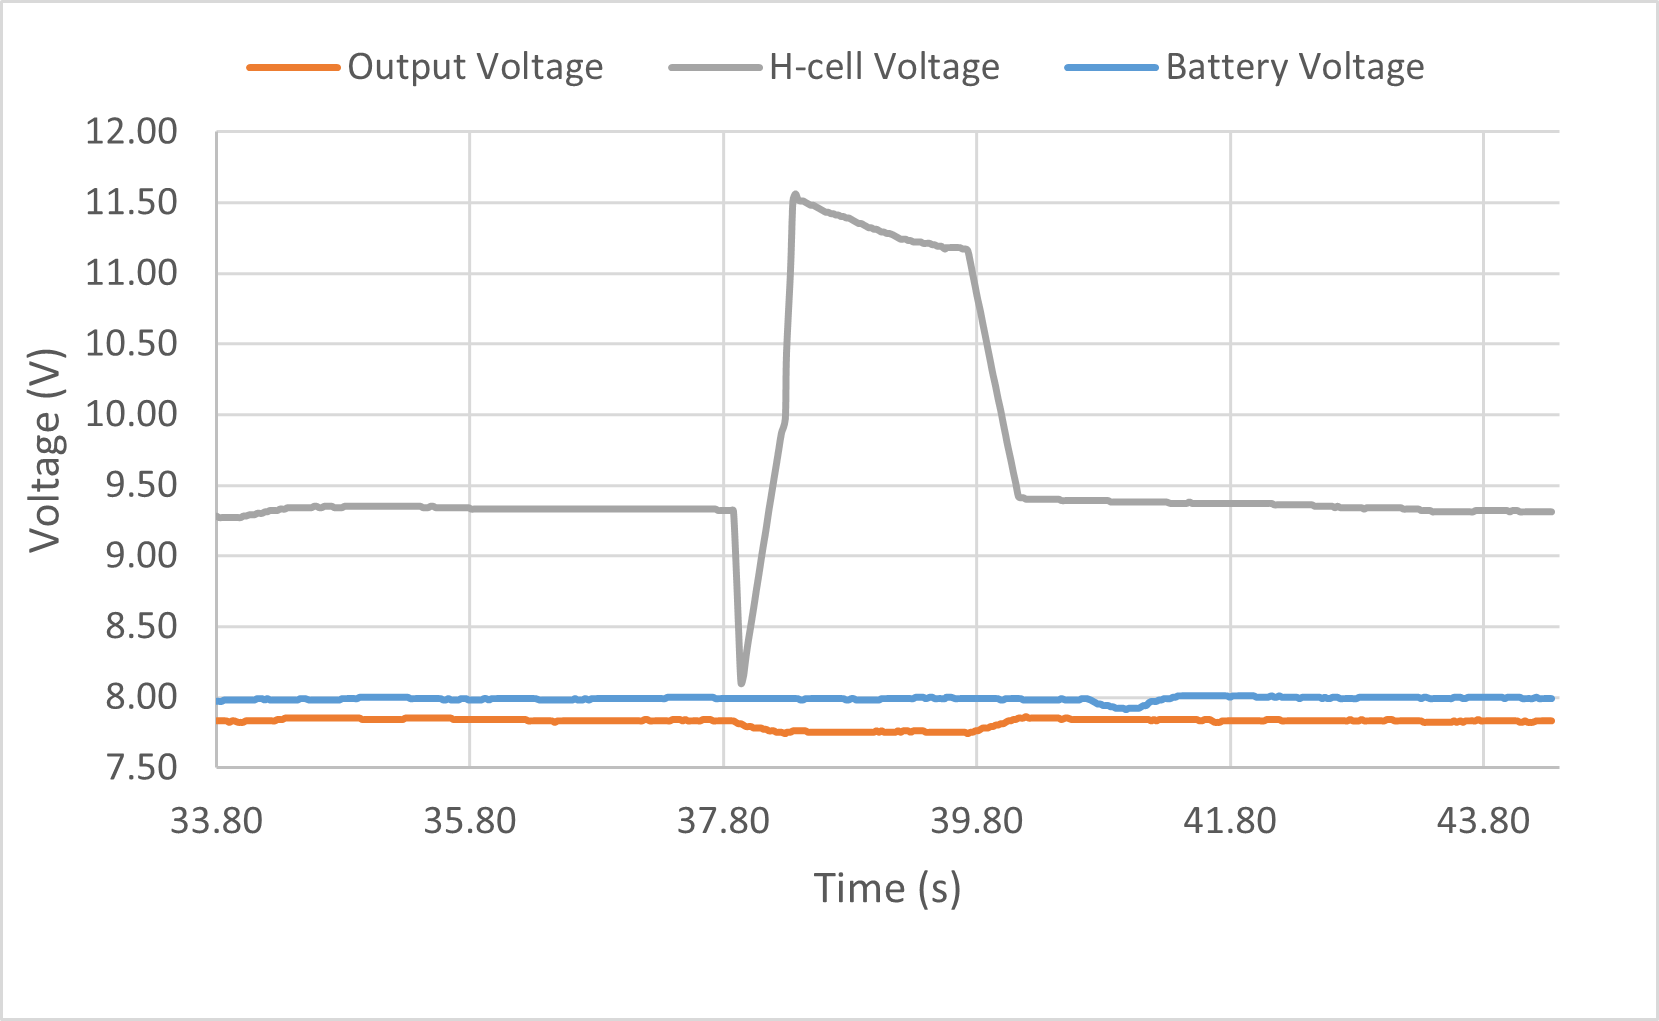
\includegraphics[width=7.5cm;]{Figures/My_figures/CASE-4 All voltages vs time 2ms.png} % Use [width=\linewidth] for full-column figure width
	\caption{Voltage characteristics at constant Speed 2 m/s}
	\label{fig:sample}
\end{figure}
\begin{figure}[h] % Single column figure
        \centering
	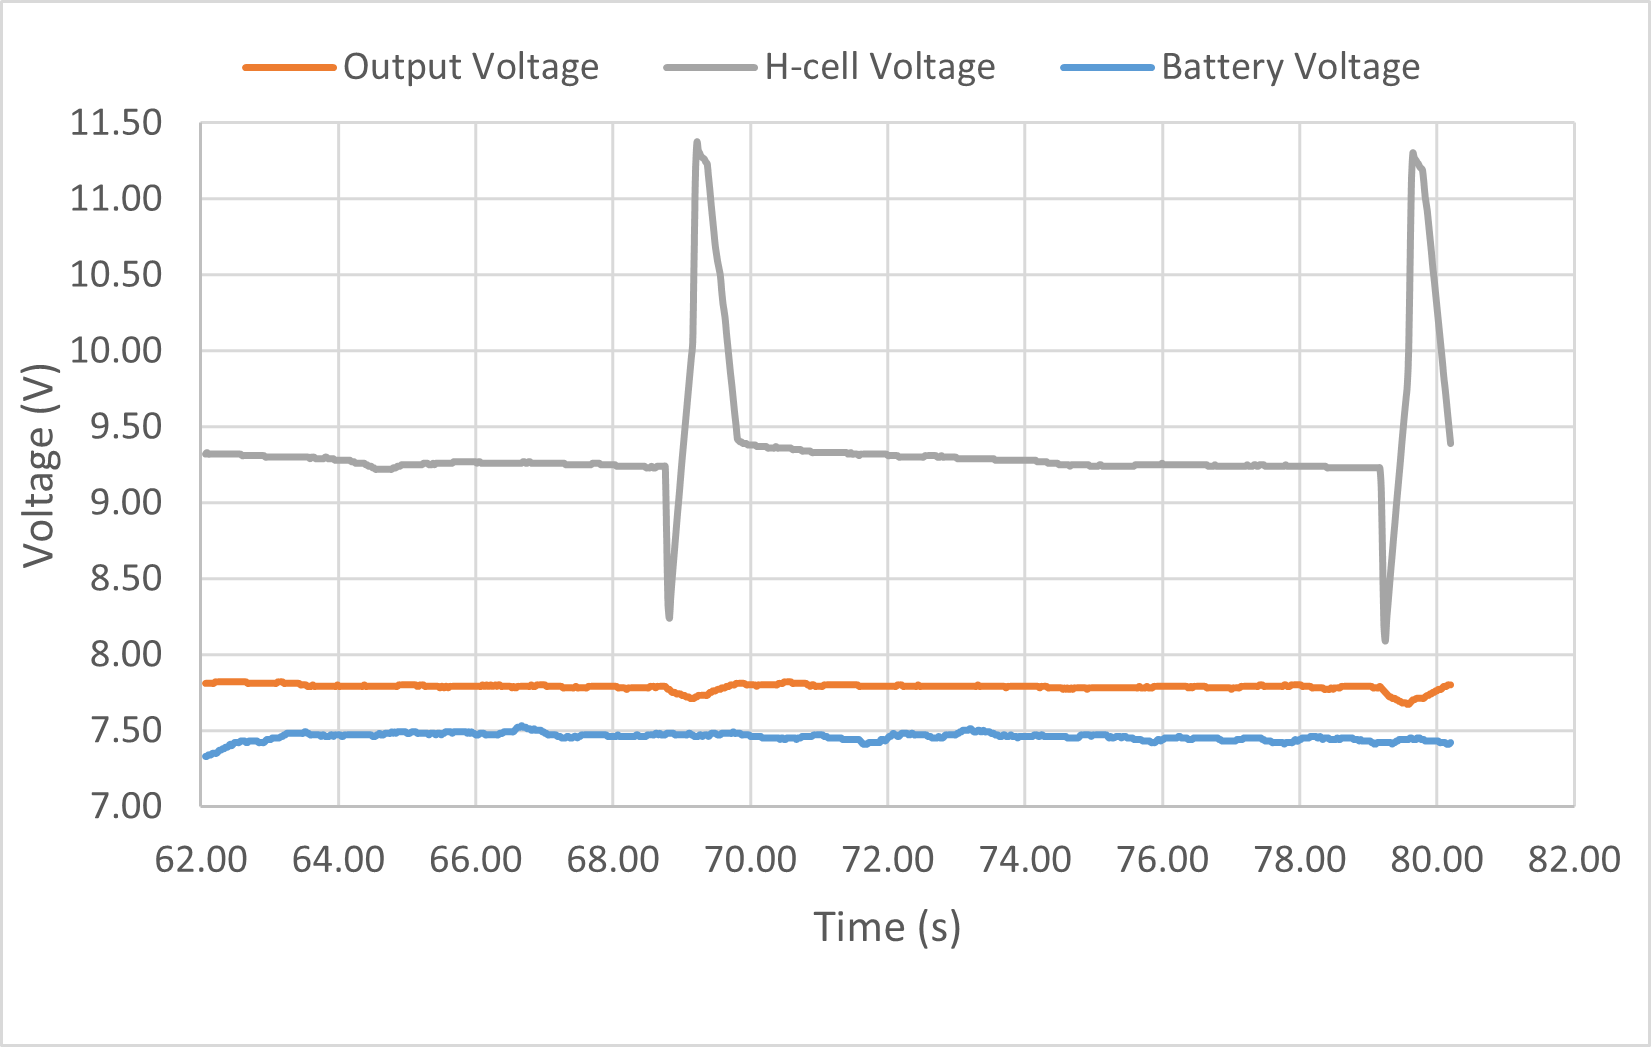
\includegraphics[width=7.5cm;]{Figures/My_figures/CASE-4 All voltages vs time.png} % Use [width=\linewidth] for full-column figure width
	\caption{Voltage characteristics at constant Speed 6 m/s}
	\label{fig:sample}
\end{figure}
The characteristic curve of the voltages with respect to time running at constant speed at 2 m/s and 6 m/s is as shown in Figures 21 and 22 respectively. At 2 m/s constant speed, the voltage of the HFC is higher as it is continuously producing more than the battery so that it needs to recharge the battery when the necessity arises. On the other hand, at the constant speed of 6 m/s the voltage of the HFC remains constant with some minor fluctuations and the battery voltage goes down for the increase in the current. The output voltage remains constant from both the battery and the HFC.



\textbf{\subsection{Braking at Constant Speed}}

In this condition, the braking force (N) is applied onto the vehicle when the vehicle is running at constant speed. The hybrid system is driven at various constant speeds for example, 8 m/s while the brakes are applied on the wheels simultaneously. The characteristic curves of the various currents with applied braking force is plotted with respect to time is as shown in below Figure-23 to investigate the system’s performance. \begin{figure}[h] % Single column figure
        \centering
	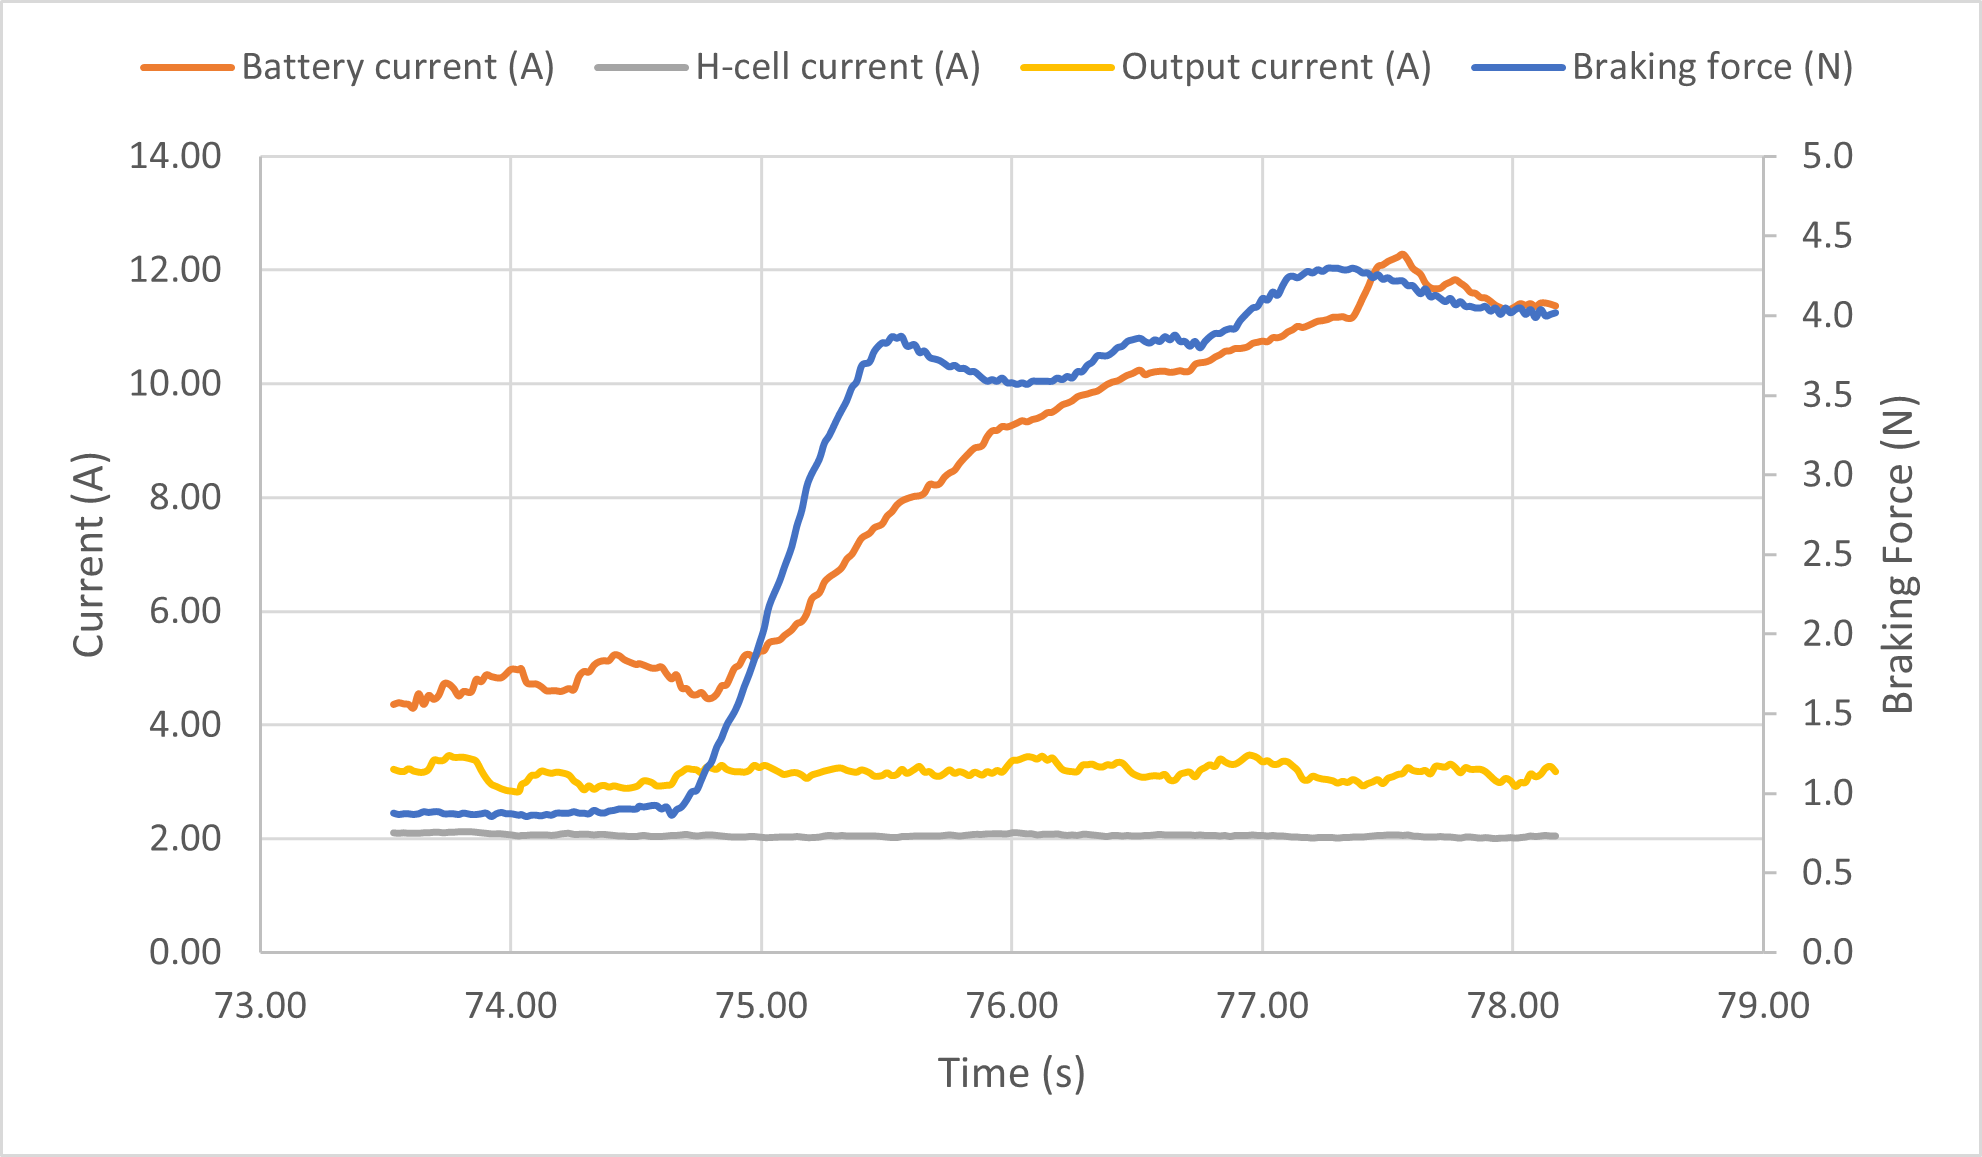
\includegraphics[width=7.5cm;]{Figures/My_figures/CASE-5 All current vs time.png} % Use [width=\linewidth] for full-column figure width
	\caption{Current characteristics - braking force applied at constant speed of 8 m/s}
	\label{fig:sample}
\end{figure}
Braking force applied gradually onto wheels to increase the torque effect on the system. Due to this, as the brake force increases, the battery current increases in order to compensate for the increased load. However, the HFC current is maintained at a constant level of approximately 2A. This shows that the braking force has almost no influence on the HFC current at this constant driving speed. The Energy management system ensures that the brake force has no influence on the HFC current. On the other hand, the output current remained maintained constant with the increase in the braking load on the system.

\begin{figure}[h] % Single column figure
        \centering
	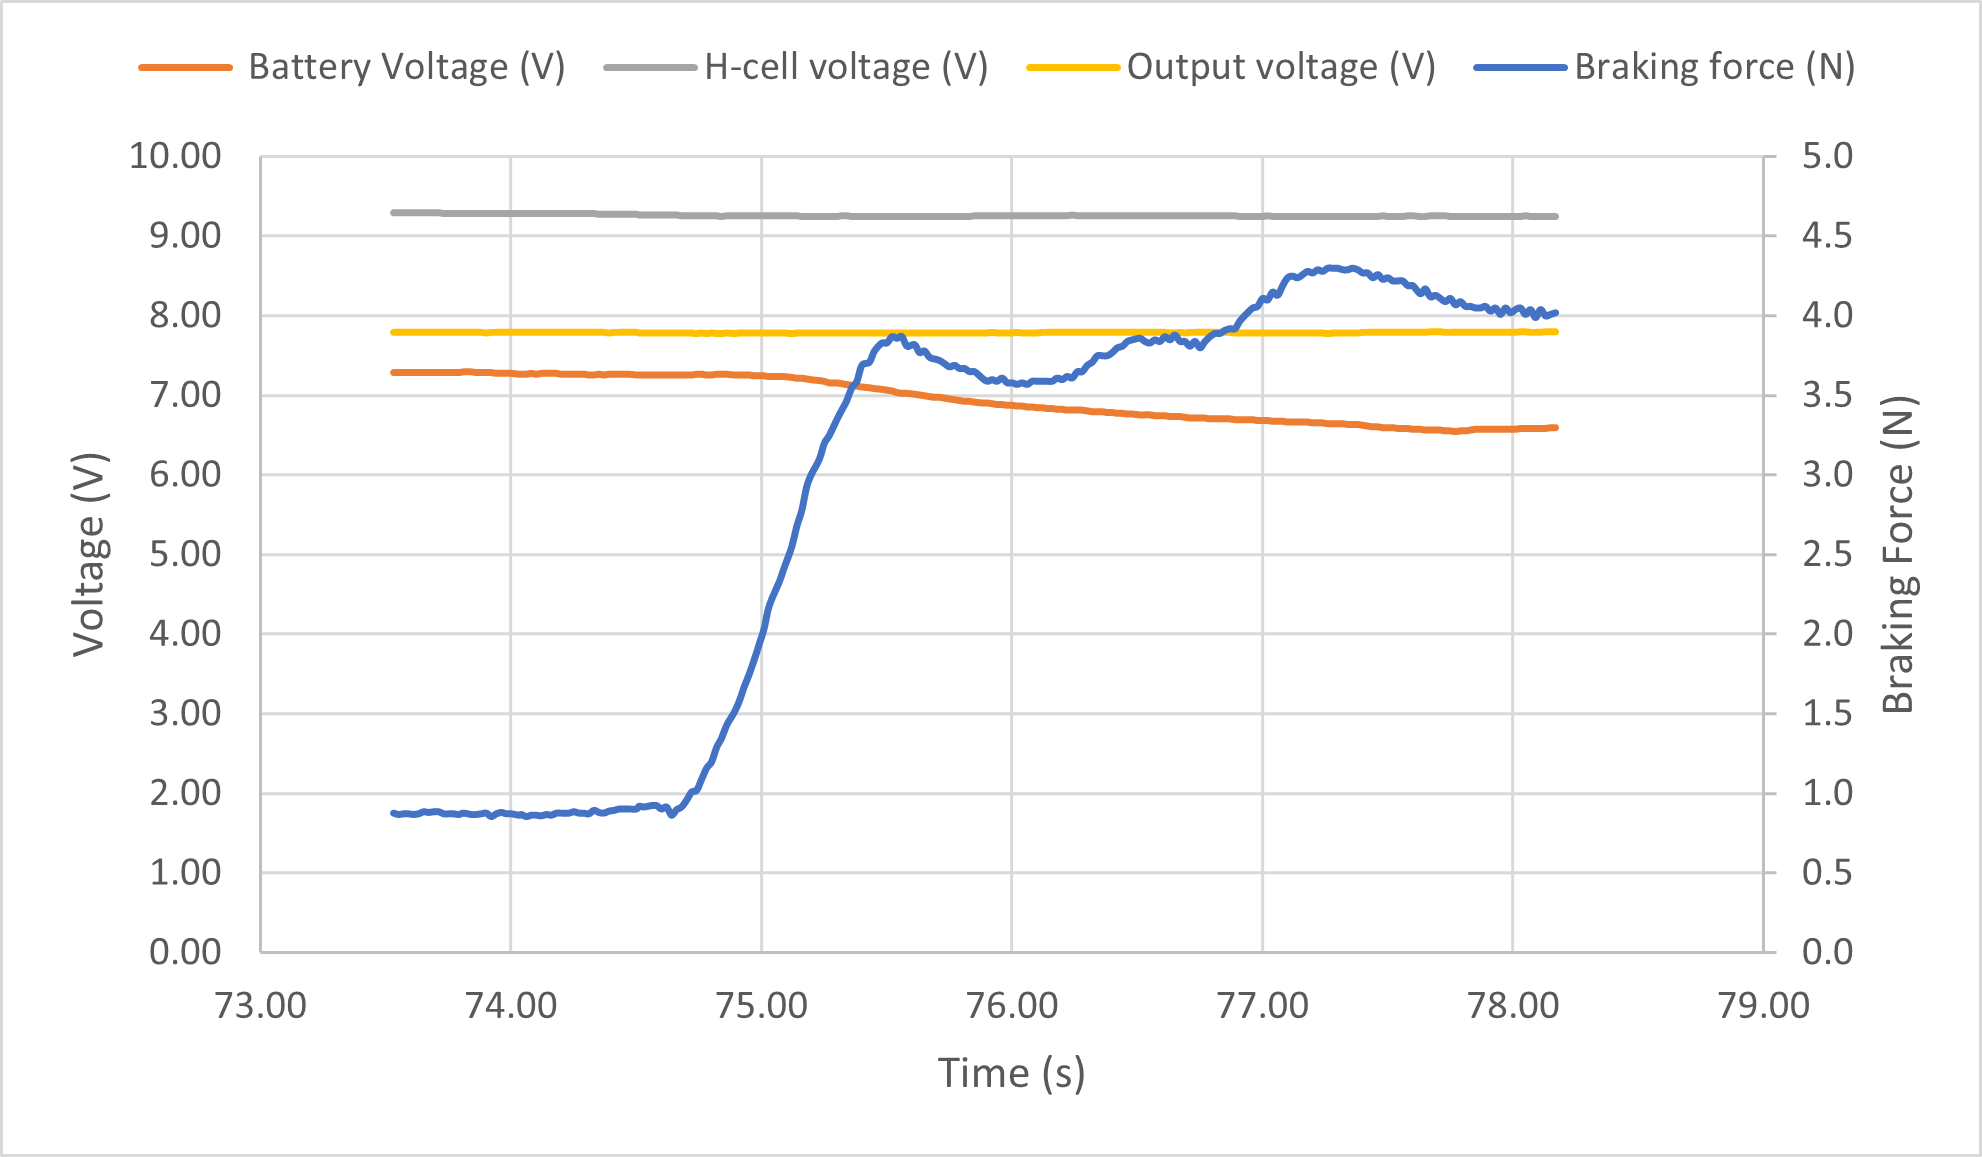
\includegraphics[width=7.5cm;]{Figures/My_figures/CASE-5 All voltages vs time.png} % Use [width=\linewidth] for full-column figure width
	\caption{Voltage characteristics - braking force applied at constant speed}
	\label{fig:sample}
\end{figure}
 Performance characteristic curves of the HFC voltage and battery voltage with braking force is as shown in below Figure-24. It is shown that braking force affects the battery voltage. As the braking force increases the battery voltage decreases, indicating that they are in inversely proportional to each other. Towards the far end of the curves, a small increase can also be seen in the battery voltage when the brake force reduces. The changes in the HFC voltage when the brake force increases remains constant. Hence, the braking force influences the battery current and voltage. 

\section{Conclusion}
Increasing carbon dioxide concentration in the atmosphere is an alarming problem and certainly needs pivotal calls-to-action to mitigate the consequences. With the advent depletion of fossil fuels, renewable fuel sources are the only way to move forward. It is complex and expensive to build, simulate, and test vehicles under various driving conditions in a 1:1 scale. This study demonstrates the performance of the hybrid propulsion system under various driving conditions.

The stand-alone analysis of the HFC signifies that the voltage reduces linearly as the current increases. Furthermore, the power is directly proportional to current upto its threshold value, after that power starts dropping. The effect of cell temperature on the voltage was systematically analysed and deduced that the fuel cell delivered a higher voltage at relatively lower temperatures such as 35-37°C in comparison to higher temperatures such as 42-45°C.

Hybrid propulsion system with a combination of battery and HFC was studied. This system was methodically analysed to define the performance of the vehicle under different driving conditions. During idling, the vehicle’s battery is charged by the HFC which is indicated by a negative current load on the battery and a positive current load on the hydrogen fuel cell. When the vehicle is gradually or rapidly accelerated, it is evident that the battery current increases simultaneously, while the hydrogen fuel cell current is maintained at an approximate constant. Therefore, it can be stated that the involvement of the hydrogen fuel cell is minimal and that the battery voltage is directly being used in acceleration immaterial of the manner of acceleration. Interestingly, when the vehicle is driven at a constant speed, the hydrogen fuel cell drives the system predominantly, while the battery is inactive. This is indicated by the high current placed on the hydrogen fuel cell and a relatively lower current placed on the battery. Therefore, in situations such as cruise-controlled driving, the hydrogen fuel cell plays a pivotal role in the mobility of the vehicle. Simulating situations such as applying brakes when the vehicle is being driven at a constant speed demonstrated that the hydrogen fuel cell current remained constant and that the battery current increases as the braking force increases.

Through this research, the characteristics of a hybrid propulsion system have been simulated, analysed, and defined. The performance curves have been illustrated for a complete understanding of the system. Although it is not perfect, the performance of this hybrid propulsion system certainly indicates a high-potential alternative to an IC engine powered vehicle. It is clear that if the limitations of the system are methodically mitigated, then it possesses all the attributes of being the most promising solution.
                                               

\section{References}
\begin{enumerate}
	\item Hydrogen Technologies – Reimund Neugebauer – Springer – 2022 
	\item Electric, Hybrid, and Fuel Cell Vehicles – Amgad Elgowainy – Springer – 2021
    \item Hydrogen in Automotive Engineering – Manfred Klell et al., Springer – 2017
    \item Fuel Cell and Hydrogen Technologies in Aviation – Can Ozgur Colpan et al., Springer – 2022
    \item H2 Engineering Kit Lab Manual – Insite Education
    \item A Comprehensive Power Management Approach for Hydrogen Fuel-cell-Based Hybrid EVs Using PID Controller – Maneesh Kumar et al., IEEE – 2023, DOI - 
    \item Experimental Study on the Steady-State Characteristics of Hydrogen Fuel Cell Engines – Kun Zhao et al., IEEE – 2022 – DOI - 10.1109/ICAPC57304.2022.00010
    \item Polymer Electrolyte Fuel Cell Durability – Felix N. Büchi et al, Springer – 2009 
    \item Muzamir Isa, Baharuddin Ismail-Characteristic Curve of a Fuel Cell, American Journal of Applied Science-2006.
    \item Xingwang Tang, Yujia Zhang, Sichuan Xu-Temperature Sensitivity characteristics of PEM fuel cell and output performance improvement based on optimal active temperature control, International Journal of Heat and Mass Transfer-2023
    \item A. Kannan, A. Kabza, and J. Scholta, “Long term testing of start-stop cycles on high temperature PEM fuel cell stack,” J Power Sources, vol. 277, pp. 312–316, Mar. 2015, doi: 10.1016/j.jpowsour.2014.11.115.
    \item B. Tanç, H. T. Arat, E. Baltacıoğlu, and K. Aydın, “Overview of the next quarter century vision of hydrogen fuel cell electric vehicles,” Int J Hydrogen Energy, vol. 44, no. 20, pp. 10120–10128, 2019, doi: 10.1016/j.ijhydene.2018.10.112.
    \item I. Pielecha, “Modeling of Fuel Cells Characteristics in Relation to Real Driving Conditions of FCHEV Vehicles,” Energies (Basel), vol. 15, no. 18, Sep. 2022, doi: 10.3390/en15186753.
    \item FCAT-30 System Adaptability – Horizon Educational 
    \item FCAT-30 Car Systems – Horizon Educational
    \item Integrating a Hydrogen Fuel Cell in a Vehicle as a Hybrid for a Sustainable Energy Application – Muhammad Amer Zahin Ahmad Dzaki et al., - Springer – 2023
    \item A review of polymer electrolyte membrane fuel cells: Technology, applications, and needs on fundamental research - Yun Wang, Ken S. Chen, Jeffrey Mishler, Sung Chan Cho, Xavier Cordobes Adroher – Elsevier – 2010
    \item Digital twin of a hydrogen Fuel Cell Hybrid Electric Vehicle: Effect of the control strategy on energy efficiency- Lorenzo Bartolucci, Edoardo Cennamo, Stefano Cordiner, Vincenzo Mulone, Ferdinando Pasqualini, Marco Aimo Boot – Science Direct- 2023- https://doi.org/10.1016/j.ijhydene.2022.11.283
    \item Experimental and numerical study of energy and thermal management system for a hydrogen fuel cell-battery hybrid electric vehicle- Gürsel Şefkat, Mert Ali Özel-Science Direct-  Volume 238, Part B- 2022 - https://doi.org/10.1016/j.energy.2021.121794
    \item Hydrogen fuel cell vehicles: Current status and future prospect- Yogesh Manoharan, Seyed Ehsan Hosseini ,Brayden Butler, Hisham Alzhahrani, Bhi Thi Fou Senior, Turaj Ashuri and John Krohn –Science Direct- 2019 - https://doi.org/10.3390/app9112296
    \item Achieving sustainable development goals through adoption of hydrogen fuel cell vehicles in India: An empirical analysis- Sidhartha Harichandan, Sanjay Kumar Kar, Rohit Bansal, Saroj Kumar Mishra- International Journal of Hydrogen Energy,Volume 48, Issue 12, 2023, Pages 4845-4859
    \item A. Jacome, D. Hissel, V. Heiries, M. Gerard, and S. Rosini, “A review of model-based prognostic for Proton Exchange Membrane Fuel Cell under Automotive Load Cycling,” in 2019 IEEE Vehicle Power and Propulsion Conference (VPPC), IEEE, Ed., 2019.
    \item B. Tanç, H. T. Arat, E. Baltacıoğlu, and K. Aydın, “Overview of the next quarter century vision of hydrogen fuel cell electric vehicles,” Int J Hydrogen Energy, vol. 44, no. 20, pp. 10120–10128, 2019, doi: 10.1016/j.ijhydene.2018.10.112.
    \item S. Ma et al., “Fuel cell-battery hybrid systems for mobility and off-grid applications: A review,” Renewable and Sustainable Energy Reviews, vol. 135, p. 110119, 2021, doi: https://doi.org/10.1016/j.rser.2020.110119.


 



 
\end{enumerate}

%----------------------------------------------------------------------------------------
%	 REFERENCES
%----------------------------------------------------------------------------------------



%----------------------------------------------------------------------------------------

\end{document}
